% Options for packages loaded elsewhere
% Options for packages loaded elsewhere
\PassOptionsToPackage{unicode}{hyperref}
\PassOptionsToPackage{hyphens}{url}
\PassOptionsToPackage{dvipsnames,svgnames,x11names}{xcolor}
%
\documentclass[
  12pt,
  titlepage]{article}
\usepackage{xcolor}
\usepackage[margin=2.5cm]{geometry}
\usepackage{amsmath,amssymb}
\setcounter{secnumdepth}{5}
\usepackage{iftex}
\ifPDFTeX
  \usepackage[T1]{fontenc}
  \usepackage[utf8]{inputenc}
  \usepackage{textcomp} % provide euro and other symbols
\else % if luatex or xetex
  \usepackage{unicode-math} % this also loads fontspec
  \defaultfontfeatures{Scale=MatchLowercase}
  \defaultfontfeatures[\rmfamily]{Ligatures=TeX,Scale=1}
\fi
\usepackage{lmodern}
\ifPDFTeX\else
  % xetex/luatex font selection
\fi
% Use upquote if available, for straight quotes in verbatim environments
\IfFileExists{upquote.sty}{\usepackage{upquote}}{}
\IfFileExists{microtype.sty}{% use microtype if available
  \usepackage[]{microtype}
  \UseMicrotypeSet[protrusion]{basicmath} % disable protrusion for tt fonts
}{}
\makeatletter
\@ifundefined{KOMAClassName}{% if non-KOMA class
  \IfFileExists{parskip.sty}{%
    \usepackage{parskip}
  }{% else
    \setlength{\parindent}{0pt}
    \setlength{\parskip}{6pt plus 2pt minus 1pt}}
}{% if KOMA class
  \KOMAoptions{parskip=half}}
\makeatother
% Make \paragraph and \subparagraph free-standing
\makeatletter
\ifx\paragraph\undefined\else
  \let\oldparagraph\paragraph
  \renewcommand{\paragraph}{
    \@ifstar
      \xxxParagraphStar
      \xxxParagraphNoStar
  }
  \newcommand{\xxxParagraphStar}[1]{\oldparagraph*{#1}\mbox{}}
  \newcommand{\xxxParagraphNoStar}[1]{\oldparagraph{#1}\mbox{}}
\fi
\ifx\subparagraph\undefined\else
  \let\oldsubparagraph\subparagraph
  \renewcommand{\subparagraph}{
    \@ifstar
      \xxxSubParagraphStar
      \xxxSubParagraphNoStar
  }
  \newcommand{\xxxSubParagraphStar}[1]{\oldsubparagraph*{#1}\mbox{}}
  \newcommand{\xxxSubParagraphNoStar}[1]{\oldsubparagraph{#1}\mbox{}}
\fi
\makeatother


\usepackage{longtable,booktabs,array}
\usepackage{calc} % for calculating minipage widths
% Correct order of tables after \paragraph or \subparagraph
\usepackage{etoolbox}
\makeatletter
\patchcmd\longtable{\par}{\if@noskipsec\mbox{}\fi\par}{}{}
\makeatother
% Allow footnotes in longtable head/foot
\IfFileExists{footnotehyper.sty}{\usepackage{footnotehyper}}{\usepackage{footnote}}
\makesavenoteenv{longtable}
\usepackage{graphicx}
\makeatletter
\newsavebox\pandoc@box
\newcommand*\pandocbounded[1]{% scales image to fit in text height/width
  \sbox\pandoc@box{#1}%
  \Gscale@div\@tempa{\textheight}{\dimexpr\ht\pandoc@box+\dp\pandoc@box\relax}%
  \Gscale@div\@tempb{\linewidth}{\wd\pandoc@box}%
  \ifdim\@tempb\p@<\@tempa\p@\let\@tempa\@tempb\fi% select the smaller of both
  \ifdim\@tempa\p@<\p@\scalebox{\@tempa}{\usebox\pandoc@box}%
  \else\usebox{\pandoc@box}%
  \fi%
}
% Set default figure placement to htbp
\def\fps@figure{htbp}
\makeatother


% definitions for citeproc citations
\NewDocumentCommand\citeproctext{}{}
\NewDocumentCommand\citeproc{mm}{%
  \begingroup\def\citeproctext{#2}\cite{#1}\endgroup}
\makeatletter
 % allow citations to break across lines
 \let\@cite@ofmt\@firstofone
 % avoid brackets around text for \cite:
 \def\@biblabel#1{}
 \def\@cite#1#2{{#1\if@tempswa , #2\fi}}
\makeatother
\newlength{\cslhangindent}
\setlength{\cslhangindent}{1.5em}
\newlength{\csllabelwidth}
\setlength{\csllabelwidth}{3em}
\newenvironment{CSLReferences}[2] % #1 hanging-indent, #2 entry-spacing
 {\begin{list}{}{%
  \setlength{\itemindent}{0pt}
  \setlength{\leftmargin}{0pt}
  \setlength{\parsep}{0pt}
  % turn on hanging indent if param 1 is 1
  \ifodd #1
   \setlength{\leftmargin}{\cslhangindent}
   \setlength{\itemindent}{-1\cslhangindent}
  \fi
  % set entry spacing
  \setlength{\itemsep}{#2\baselineskip}}}
 {\end{list}}
\usepackage{calc}
\newcommand{\CSLBlock}[1]{\hfill\break\parbox[t]{\linewidth}{\strut\ignorespaces#1\strut}}
\newcommand{\CSLLeftMargin}[1]{\parbox[t]{\csllabelwidth}{\strut#1\strut}}
\newcommand{\CSLRightInline}[1]{\parbox[t]{\linewidth - \csllabelwidth}{\strut#1\strut}}
\newcommand{\CSLIndent}[1]{\hspace{\cslhangindent}#1}



\setlength{\emergencystretch}{3em} % prevent overfull lines

\providecommand{\tightlist}{%
  \setlength{\itemsep}{0pt}\setlength{\parskip}{0pt}}



 


\usepackage{booktabs}
\usepackage{longtable}
\usepackage{array}
\usepackage{multirow}
\usepackage{wrapfig}
\usepackage{float}
\usepackage{colortbl}
\usepackage{pdflscape}
\usepackage{tabu}
\usepackage{threeparttable}
\usepackage{threeparttablex}
\usepackage[normalem]{ulem}
\usepackage{makecell}
\usepackage{xcolor}
\usepackage{authblk}
\renewcommand\Affilfont{\small\itshape}
\renewcommand\Authfont{\normalsize}
\author[1]{Adam Dennett\thanks{a.dennett@ucl.ac.uk, ORCID: 0000-0002-7493-3276}}
\author[1]{Beatrice Taylor\thanks{beatrice.taylor@ucl.ac.uk, ORCID: 0000-0002-3630-5047 }}
\author[3]{Dan Campbell-Meiklejohn\thanks{daniel.cm@sussex.ac.uk, ORCID: 0000-0002-8916-265X}}
\affil[1]{Bartlett Centre for Advanced Spatial Analysis, University College London}
\affil[3]{School of Psychology, University of Sussex}
\renewcommand{\author}[2][]{}
\renewcommand{\and}{}
\makeatletter
\@ifpackageloaded{caption}{}{\usepackage{caption}}
\AtBeginDocument{%
\ifdefined\contentsname
  \renewcommand*\contentsname{Table of contents}
\else
  \newcommand\contentsname{Table of contents}
\fi
\ifdefined\listfigurename
  \renewcommand*\listfigurename{List of Figures}
\else
  \newcommand\listfigurename{List of Figures}
\fi
\ifdefined\listtablename
  \renewcommand*\listtablename{List of Tables}
\else
  \newcommand\listtablename{List of Tables}
\fi
\ifdefined\figurename
  \renewcommand*\figurename{Figure}
\else
  \newcommand\figurename{Figure}
\fi
\ifdefined\tablename
  \renewcommand*\tablename{Table}
\else
  \newcommand\tablename{Table}
\fi
}
\@ifpackageloaded{float}{}{\usepackage{float}}
\floatstyle{ruled}
\@ifundefined{c@chapter}{\newfloat{codelisting}{h}{lop}}{\newfloat{codelisting}{h}{lop}[chapter]}
\floatname{codelisting}{Listing}
\newcommand*\listoflistings{\listof{codelisting}{List of Listings}}
\makeatother
\makeatletter
\makeatother
\makeatletter
\@ifpackageloaded{caption}{}{\usepackage{caption}}
\@ifpackageloaded{subcaption}{}{\usepackage{subcaption}}
\makeatother
\usepackage{bookmark}
\IfFileExists{xurl.sty}{\usepackage{xurl}}{} % add URL line breaks if available
\urlstyle{same}
\hypersetup{
  pdftitle={Pulling the Right Lever: School Attainment, Open Data Analytics and Local Education Policy in England},
  pdfauthor={Adam Dennett; Beatrice Taylor; Dan Campbell-Meiklejohn},
  pdfkeywords={school attainment, education policy, school
absence, disadvantage gap, multilevel modelling, open data},
  colorlinks=true,
  linkcolor={blue},
  filecolor={Maroon},
  citecolor={Blue},
  urlcolor={Blue},
  pdfcreator={LaTeX via pandoc}}


\title{Pulling the Right Lever: School Attainment, Open Data Analytics
and Local Education Policy in England}
\author{Adam Dennett \and Beatrice Taylor \and Dan Campbell-Meiklejohn}
\date{2026-09-04}
\begin{document}
\maketitle
\begin{abstract}
The UK government's 2026 White Paper targets halving the disadvantage
attainment gap. Achieving this requires local education authorities to
understand the drivers of attainment in their areas, but challenges in
evidence synthesis and locally relevant data analytics mean the risk of
pulling the wrong policy lever is high. Using linear mixed-effects
models fitted to 4-years of DfE data, we show school-level Attainment 8
is highly predictable. Focusing on Brighton and Hove, where 2024
secondary admissions changes were premised on the idea that
disadvantaged student attainment could be improved through even more
social mixing in the school system, our analysis suggests that through
omitted variables, non-linearities and counter-intuitive relationships,
the policy is unlikely to deliver the targeted gains, while the wider
literature on long school commutes points to social and educational
costs not adequately considered. The city has the second-worst absence
rate in England in 2024-25 (and among the worst throughout the period),
and our modelling indicates improving attendance would be the most
impactful single policy lever, particularly for disadvantaged pupils. We
also introduce a school-level value-added view that lets parents and
policy makers assess how a school performs above its inherited intake
characteristics, and a policy simulator tool to bridge the gap between
open data and accessible, contextualised intelligence.
\end{abstract}


\section{Introduction}\label{introduction}

Pupil outcomes, including attainment, are a recurrent policy theme given
the established links to individual life outcomes (Farquharson et al.
2024) and our collective national success through measures such as
economic productivity (Grant 2017). The UK Government's 2026 schools
white paper (DfE 2026) sets ambitious targets including halving the
disadvantage attainment gap, improving attendance, reforming admissions
and tackling place-based disadvantage. These ambitions will require
local education authorities (LEAs) to understand the specific drivers in
their areas and choose interventions accordingly.

Focusing on the secondary school attainment, this paper argues that the
Department for Education's (DfE) open data provides most of the raw
materials needed for such nuanced localised understanding, but a crucial
gap exists between data availability and accessible, contextualised
intelligence for decision makers. We demonstrate this through an
analysis of school-level attainment across England, combined with a case
study of Brighton and Hove where a policy direction would be predicted
by our model, to potentially do more harm than good.

Brighton and Hove provides a particularly instructive case. The city
already has a distinctive admissions landscape featuring catchment areas
with a lottery tie-break for oversubscribed schools, introduced
following a secondary school closure in 2005 (Allen et al. 2013), and an
admissions priority for Free-School-Meal (FSM)-eligible pupils across
its community schools. In 2024, the council launched proposals to reduce
Published Admission Numbers at popular central-catchment schools,
reserve places for out-of-catchment children in those catchments ahead
of in-catchment children, and redraw catchment boundaries. The proposals
were promoted on the premise that attainment in the city was `driven by
economic advantage' and that redistributing pupils would narrow the
attainment gap. The public response was overwhelmingly negative, yet
parents and schools lacked the tools to challenge the proposals
effectively and the core policy direction persisted, albeit slightly
watered down.

Raw data on the attainment gap, without context, was presented to the
city alongside statements correlating concentrations of disadvantage
with lower attainment. The gap was framed as a unique failure requiring
urgent action; the second-order impacts of the proposed interventions -
longer school journeys, displacement from local communities, effects on
well-being - were not scrutinised in depth. Our modelling addresses a
critical blind spot in local decision-making: without the ability to
account for structural factors like absence and prior attainment,
councillors and citizens were unaware that, \emph{after controlling for
absence in particular}, Brighton and Hove was already among the
highest-performing LEAs nationally for taking students beyond those
factors - ranking 15th of 151 for disadvantaged pupils and 4th for
non-disadvantaged pupils. As we show later, that conditional ranking is
itself a measure of how much the city's severe absence problem is
costing its disadvantaged pupils: set absence aside and the schools look
exceptional; leave it in the ledger and the city is ordinary. These
insights come from the analysis of open data presented in this paper and
carried out after the consultation had closed. However, with more timely
analysis and with this knowledge, the approach to improving outcomes for
disadvantaged pupils in the city could have been more effective and
different questions asked: ``what can we learn from what the city is
doing right?'' and ``would asking pupils to travel out of their
communities to schools jeopardise this success?'' Some rapidly-produced
analysis was put into the public domain by some of the authors of this
paper\footnote{\url{https://osf.io/x82j3/overview} (see `about.html` in
  `supplementary.zip`)}, but as a response to, not a contribution to,
policy formation.

The discussions that led to this paper took place over an 18-month
period spanning the 2024 and 2025 admissions consultations and involved
a diverse group of parents, academics, policy practitioners and school
governors. We do not claim our model is optimal or novel - the variables
and effects are very similar to those reported by Macleod et al. (2015)
over a decade ago. Our intention is to show that with freely available
open data and a small set of well-chosen variables, it is possible to
build a model explaining close to 80\% of the variation in school-level
Attainment 8, and then to use it to answer locally targeted questions
such as: `is changing the social mix in schools likely to improve
disadvantaged pupil attainment?', `what is the most important factor
affecting attainment in a particular LEA?', and `which schools are doing
better or worse than expected?'. We report effects in GCSE-point units
rather than standard deviations so that they have more direct meaning
for policy makers.

Before examining the Brighton and Hove proposals specifically later in
the paper, we wish to be explicit about the scope of our argument. Our
models measure attainment outcomes only; they cannot speak to the
broader social, civic and developmental value of diverse school
communities, which we do not dispute. We are also aware that our
findings regarding concentrations of disadvantaged students could be
read selectively to justify resistance to integration efforts in general
--- that is not our argument. Our claim is specific: in this city, at
this time, with this evidence base, the proposed mixing intervention was
not the most impactful lever available for disadvantaged student
attainment, and carried costs the consultation did not adequately weigh.

The paper proceeds as follows. We briefly review the literature on
secondary school attainment drivers, then outline our modelling approach
using DfE open data. We present results showing which factors matter
most and how they interact, before applying these findings to Brighton
and Hove. We conclude with implications for local and national education
policy.

\section{Literature review: factors affecting pupil
attainment}\label{literature-review-factors-affecting-pupil-attainment}

\subsection{Socio-economic background and
disadvantage}\label{socio-economic-background-and-disadvantage}

The Education Policy Institute's annual reports document that by the
time pupils sit their GCSEs (the General Certificate of Secondary
Education - the exam most students in England sit at age 16),
disadvantaged pupils are on average around 18 months of learning behind
their more affluent peers, a gap that narrowed modestly after 2011 but
partially reversed following the COVID-19 pandemic (Tuckett et al.
2023). It is this `attainment-gap' which has remained stubbornly
persistent for many years and that the recent government white paper has
resolved to try and tackle. The size of the gap and the reasons behind
it are complex and vary from place to place, but its existence has
spawned large volumes of literature delving into disadvantage and
attainment (for wider reviews and evidence syntheses, see e.g. Stopforth
and Gayle (2025); Macleod et al. (2015); Tuckett et al. (2023)).

Free School Meal (FSM) eligibility serves as the standard proxy for
disadvantage, though its limitations are well established. For example,
Stopforth and Gayle (2025) demonstrate that finer-grained measures of
parental social class reveal persistent attainment gaps that FSM-based
analyses tend to understate, with the thresholds for FSM eligibility low
enough that many students who might otherwise be classed as
disadvantaged, are not included in these statistics. Despite this,
because eligibility for Free School Meals is regularly recorded at pupil
and school levels, it is frequently used as a proxy.

Inequalities in GCSE outcomes are substantially mediated by prior
attainment at National Curriculum Key Stage 2 (KS2 - the latter stages
of primary school from ages 7 to 11\footnote{Details of English National
  Curriculum Key Stages \url{https://www.gov.uk/national-curriculum}}),
reflecting accumulated inequalities from before secondary school
(Stopforth and Gayle 2025). Gorard and Siddiqui (2019) show that the
duration of disadvantage is a stronger predictor than disadvantage at
any single point, and propose that pupils do worse in schools with
higher concentrations of disadvantage, estimating improvements of
0.05--0.15 standard deviations (approximately one GCSE grade in one
subject) from greater social mixing. They argue this can be achieved at
`almost no cost' - a conjecture that overlooks real-world consequences
for communities, particularly where local social geographies mean
de-concentration requires children travelling long distances.

\subsection{Attendance}\label{attendance}

School attendance is among the strongest predictors of attainment and
this comes through strongly in the literature. DfE analysis of 2018/19
data (DfE 2022) documents a stark gradient: among persistently absent
pupils, only 35.6\% achieved a standard pass in English and Maths,
compared with 83.7\% among those with no recorded absences. It is also
cited as one of the main factors in pushing down attainment for
disadvantaged pupils by Macleod et al. (2015). More recent analysis
finds that pupils with near-perfect attendance were 1.9 times as likely
to achieve a grade 5 pass compared with otherwise similar pupils
attending 90--95\% of the time (DfE 2025a). Dräger et al. (2024), using
the 1970 British Cohort Study, find that absences at age 10 are
associated with lower educational attainment in adulthood. The Social
Mobility Commission (Riordan et al. 2021) conclude that the correlation
between attendance and progress is `most likely to be causal'.

Post-pandemic persistent absence has risen sharply, from around 10.5\%
pre-pandemic to approximately 21.9\% in secondary schools by 2023/24,
with rates for FSM-eligible pupils around 32\% (DfE 2025b). This
compounds the challenge of disentangling school-level from pupil-level
effects.

How far attendance is amenable to \emph{school-level} action is an
important question. Some of the variation reflects school practice -
pastoral systems, attendance follow-up and ethos - but a substantial
share is driven by circumstances beyond the school gate: family poverty,
physical and mental ill-health, special educational needs, caring
responsibilities, and the broader adversities that depress attainment
through multiple channels (Houtepen et al. 2020; Rakesh et al. 2025).
The steep, largely exogenous rise in absence since the pandemic
underlines how much of the recent problem sits outside any individual
school's control. This distinction - between the intake-driven component
of absence and the smaller portion a school can itself move - is central
to how absence should be interpreted as a policy lever, and we make it
explicit in our modelling in section 5.5. It also implies that
authority-wide improvement is unlikely to come from school-led
practice-sharing alone, and more probably requires strategic,
council-led, cross-departmental action spanning health, children's
services and family support alongside schools.

\subsection{Other factors}\label{other-factors}

Ethnic inequalities are persistent (Gillborn et al. 2017), though Gorard
et al. (2025) show these are substantially reduced when controlling for
pupil-level characteristics. The under-performance of disadvantaged
White British pupils, particularly boys, has attracted policy attention,
with causes contested between place-based deprivation and cultural
factors (Strand 2021; Commons Education Committee 2021).

School-level selectivity inflates raw performance metrics. Anders et al.
(2024) find that the private school premium effectively disappears once
socio-economic background is controlled for. Burgess et al. (2018) show
grammar schools reinforce socio-economic stratification without overall
attainment benefits.

Workforce factors including effective leadership (Zuccollo et al. 2023),
teaching quality (Burgess et al. 2023), and teacher retention (Gibbons
et al. 2018; Menzies 2023) contribute to variation in attainment, with
effects felt most acutely by disadvantaged students (Allen et al. 2018).
The `London Effect' (the apparent boost to attainment for disadvantaged
pupils who live in the Capital) (Ross et al. 2020) reflects a localised
concentration of agency factors - parental expectations, homework hours,
lower unauthorised absence - rather than a purely geographic phenomenon.

The factors affecting attainment are multifaceted and interrelated, and
many drivers are well-established. With so many concurrently relevant
predictors, however, it is difficult to judge their relative importance
in any specific context. What is required is an analysis combining as
many drivers as possible, so that their relative influences,
interactions, and mediation pathways can be assessed concurrently -
which is where we now turn.

\section{Data and methods}\label{data-and-methods}

\subsection{Data}\label{data}

The DfE publishes extensive open data on schools via its statistical
services. We assembled a panel dataset covering the four post-COVID
academic years (2021--22 to 2024--25), linking school performance,
absence, pupil population, workforce and Ofsted data. Data
pre-processing details are available in the supplementary
material.\footnote{Supplementary material:
  \href{https://osf.io/x82j3/overview}{https://osf.io/x82j3/overview
  (see `index.html` in `supplementary.zip`)} - with links through to the
  source code on Github.} The full panel comprises 13,419 school-year
observations from 3,523 academies and maintained schools across 152
LEAs. Independent schools, colleges and `special schools' (those
catering more for pupils with special educational needs and
disabilities) are excluded. After the exclusion of cases with missing
predictor values or imputation of those values required for the
log-linear specification (principally missing workforce or Ofsted data
in 2024-25, together with KS2 prior attainment, which is not published
for that year because the relevant cohort's primary assessments were
cancelled during the pandemic - see section 3.2\footnote{missing data
  and imputation:
  \href{https://osf.io/x82j3/overview}{https://osf.io/x82j3/overview
  (see `data\_overview.html\#missing-data` in `supplementary.zip`)}}),
the analysis sample used in the models is approximately 12,200
observations. All data are school-level aggregates; interpretations
relate to this level of aggregation.

\subsection{Model specification}\label{model-specification}

We fit multilevel linear mixed effects models (LMEs) with schools nested
within LEAs within regions (Snijders 2012). The outcome is
log-transformed Attainment 8 (for all, disadvantaged and
non-disadvantaged pupils), the measure of interest cited in the DfE
(2026) white paper. We have selected Attainment 8 over Progress 8 as we
want to assess the influence and interaction variables like prior
attainment on other predictor variables, not just as a partial outcome.
Because the outcome is on the log scale, coefficients for
log-transformed predictors represent elasticities. We should be clear
that the log transformation is \emph{not} applied uniformly to every
predictor: only the four skewed, strictly-positive count-and-rate
variables - the disadvantage, absence and EAL percentages and teacher
sickness days - enter in logged form, chosen on the basis of visual fit
and the interpretability of elasticities. The remaining predictors,
including mean KS2 prior attainment, the segregation index and the
workforce proportions, enter linearly. This variable-by-variable choice,
together with supporting diagnostics (component-plus-residual plots and
a comparison of logged, linear and spline treatments), is documented in
the supplementary material.

The model specification is:

\[\log(\text{ATT8}_{ij}) = \beta_0 + \sum_{k=1}^{9} \beta_k \, x_{kij} + u_{\text{year}} + u_{\text{Ofsted}} + u_{\text{region}} + u_{\text{LA|region}} + \varepsilon_{ij}
\]

where \(i\) indexes schools, \(j\) indexes year-observations, the
\(\beta_k\) are fixed-effect coefficients, and the \(u\) terms are
random-effect intercepts for year, Ofsted rating, region, and LEA nested
within region.

Fixed-effect predictors comprise: log(\% KS4 pupils who are
disadvantaged - \% FSM), log(\% overall absence - \% Absence), log(\%
pupils with English as an additional language - \% EAL), mean KS2 prior
attainment (the cohort's average KS2 scaled score, centred at the
national standard of 100), selective admissions (dummy), Gorard
Segregation Index (LA-level), teacher retention rate, leadership pay
proportion, and log(teacher sickness days).

The selective-admissions variable is the DfE's own performance-tables
admissions classification, and within our state-funded sample it
distinguishes three groups: wholly \emph{selective} state grammar
schools that admit by an entrance test (166 schools, 4.8\% of the
sample); non-selective schools located in otherwise selective areas (234
schools, the reference category - we note for those not familiar with
the English system that following reforms some decades ago, only some
LEAs in England still have selective grammar schools); and all other
non-selective schools (the remaining \textasciitilde88\%). The estimate
we report is therefore the effect of \emph{full} academic selection,
benchmarked against non-selective schools whose intakes are shaped by
the same local grammar systems. It does not capture partial selection,
banding, aptitude-based selection or faith-based oversubscription
criteria, all of which fall within the `other non-selective' category
and are consequently unmeasured here; faith schools in particular are
not separately identified in the main model.

There are two points relating to the prior-attainment variable that need
highlighting. Firstly, we control for prior attainment using the
cohort's \emph{mean KS2 scaled score}, and for the final year of our
panel no observed prior-attainment data exists at all. Because the KS2
tests and assessments of 2019-20 and 2020-21 were cancelled during the
pandemic, the cohorts reaching the end of KS4 in 2024-25 and 2025-26
have no KS2 results of any kind; the DfE accordingly publishes neither
prior-attainment measures nor Progress 8 for those years.\footnote{Department
  for Education, \emph{Key stage 4 performance}: ``It is not possible to
  calculate Progress 8 for academic years 2024/25 and 2025/26. This is
  because there is no KS2 prior attainment data available to use to
  calculate Progress 8 when the relevant cohorts reach the end of KS4 as
  primary tests and assessments were cancelled in academic years 2019/20
  and 2020/21 due to COVID-19 disruption.''
  \url{https://explore-education-statistics.service.gov.uk/find-statistics/key-stage-4-performance}}
For 2024-25 we therefore carry forward each school's most recently
observed value (or, where that is unavailable, its mean across observed
years), and the affected rows are flagged in the panel (see
Supplementary material\footnote{See data overview for details
  \href{https://osf.io/x82j3/overview}{https://osf.io/x82j3/overview
  (see `data\_overview.html` in `supplementary.zip`)}} for methods and
diagnostic plots). Secondly, because we lack pupil-level data, prior
attainment is corrected only at the school level; this is a coarser
adjustment than a pupil-and-school-level correction would provide, and
therefore we can't rule out some confounding of the intake coefficients
where a common cause exists. We return to this limitation later in the
paper.

An earlier version of this analysis controlled for prior attainment
using only the \emph{percentage of pupils with low KS2 prior
attainment}. In this iteration we look at the mean KS2 score. This
implications of this change are discussed below.

We fit separate models for overall Attainment 8, disadvantaged-pupil
Attainment 8, and non-disadvantaged-pupil Attainment 8, as both panel
models (all four years) and individual year models. Models were
estimated using the \texttt{lme4} package in R with Restricted Maximum
Likelihood estimation.

Variable selection was informed by the literature review and by the
policy narrative in Brighton and Hove, where segregation featured
prominently in the council justification. Full details of the variables
and the full analysis panel can be found in the supplementary material
\footnote{See data overview for details
  \href{https://osf.io/x82j3/overview}{https://osf.io/x82j3/overview
  (see `data\_overview.html` in `supplementary.zip`)}}.

\section{Results}\label{results}

\subsection{Model fit}\label{model-fit}

The models explain a substantial proportion of variance in school-level
Attainment 8. In order that these fits are more intuitive for those used
to interpreting OLS regression models, we use the method described by
Nakagawa and Schielzeth (2013) and Nakagawa et al. (2017) to calculate
indicative \(R^2\) values proxying the proportion of Attainment 8
variance explained by each model. For all pupils, the conditional
\(R^2\) (fixed plus random effects) is 0.78, with marginal \(R^2\)
(fixed effects alone) of 0.65. For disadvantaged pupils the conditional
\(R^2\) is 0.73; for non-disadvantaged pupils, 0.8. School-level
attainment is remarkably predictable from these structural factors,
which makes them very useful for exploring the effectiveness of local
policy levers.

\subsection{Stepwise decomposition}\label{stepwise-decomposition}

\emph{{[}Table 1: Stepwise progression to the full multilevel model for
overall Attainment 8. --- about here{]}}

The stepwise progression in Table~\ref{tbl-stepwise} reveals the
mediating structure among the key predictors. In Model 1, we start with
the \% KS4 pupils who are disadvantaged (\%FSM for short) as the only
predictor - mainly as this was the variable that has dominated the
policy discussion in Brighton and Hove in recent years, leading to the
2023 FSM priority policy and the 2024 mixing policy. the FSM coefficient
is --0.201 and statistically significant, on its own accounting for
almost 40\% of the variation in Attainment 8 across schools in England.
However, adding absence in Model 2 halves it to --0.122. Absence shares
explanatory power attributed to deprivation, reducing the coefficient of
\%FSM, and adds further explanation, together they now account for over
60\% of the variation in Attainment 8 scores. Adding prior attainment in
Model 3 reduces both FSM and absence coefficients further. By Model 3,
with just three variables, close to 70\% of attainment variation is
explained.

Ranking these three predictors by importance needs more care than it
might appear, and it is worth being explicit about why. The t-values in
Model 3 (\% absence -60.5, mean KS2 58.2, \% FSM -21.0) describe how
precisely each coefficient is estimated once the other two are held
constant --- that is, each variable's \emph{unique} contribution. But
these three variables are strongly correlated with one another (\% FSM
with mean KS2 at -0.69, \% absence with mean KS2 at -0.59), so a great
deal of the variance they explain is shared between them rather than
belonging to any one. A variable that shares heavily with the others
will have a modest t-value even where it accounts for a large share of
attainment on its own, and t-values therefore cannot settle which factor
matters most.

Two measures that can apportion the shared variance point the same way
as each other. Taken on its own, mean KS2 explains 59\% of the variation
in Attainment 8, absence 50\% and \% FSM 39\%. Apportioning the shared
variance more formally, by averaging each variable's contribution across
every possible order in which the three could enter the model (the
Shapley or LMG decomposition (Grömping 2007)), gives mean KS2 42\% of
the explained variance, absence 36\% and \% FSM 23\%.

Prior attainment, then, is the largest single source of variation in
school-level attainment, with absence close behind --- consistent with
the standardised coefficients we report in section 4.3. The point that
matters for policy survives every one of these measures:
\textbf{concentrations of disadvantage come last on all three}, whether
judged by unique contribution, by explanatory power alone, or by
apportioned share. We return in section 4.3 to what follows from this,
and in particular to the distinction between a factor that is large and
a factor that can be acted upon.

Before we get to Model 4, at this point, it is worth noting that in this
iteration of the analysis we switch from low KS2 prior attainment to
mean KS2 score - the difference materially affects two of our estimates.
The low-attainment share measures only the bottom of a school's intake
distribution: it records how many pupils arrived already behind, but
says nothing about how many arrived ahead. Two schools with identical
proportions of low prior attainers can have very different intakes
across the rest of the attainment spectrum. A model controlling only for
the low-attainment share cannot distinguish them, and so systematically
under-adjusts for schools whose advantage lies at the \emph{top} of the
distribution. Mean KS2 score, contrastingly, reflects the whole
distribution - both tails - and produces a better model fit (a reduction
in AIC of over 500 for the all-pupil model); once it is included, the
low-attainment share adds nothing further (t = -0.45).

This matters for the interpretation of the analysis. The coefficient on
concentrations of disadvantage falls by roughly a \emph{quarter} for all
pupils, because the low-attainment share had been leaving part of the
intake difference between high- and low-FSM schools unmeasured, and the
FSM variable had been absorbing it. Properly controlled, disadvantage
concentration is an even \emph{weaker} predictor of attainment than our
earlier specification implied. For disadvantaged pupils specifically,
the positive coefficient on disadvantage concentration becomes both
larger and far more clearly distinguishable from zero (\emph{t} rising
from 2.1 to 5.6) - disadvantaged pupils in high disadvantage schools are
even more positively affected by this than our earlier specification led
us to believe. The absence coefficient, by contrast, barely moves -
under 3\% in either pupil group - so the paper's central finding is
unaffected by the choice. The practical lesson is that in modelling KS4
outcomes it is not sufficient to ask how many pupils arrived behind; how
many arrived ahead matters just as much, and controlling just for the
low prior attainment tale has the effect of quietly over-crediting
schools for intake advantages they did not create.

We should add a note of caution relating to interpretations following
this improvement. Prior attainment at Key Stage 2 is not independent of
disadvantage: a large chunk of prior attainment actually reflects the
inequalities a child has already experienced before secondary school
ever begins (Stopforth and Gayle 2025; Gorard and Siddiqui 2019). A
variable that captures the whole intake distribution therefore absorbs
correspondingly more of the poverty signal than one that captures just
the low attainment tail - which is precisely why the disadvantage
coefficient attenuates when we make the switch from low to mean KS2
attainment. The coefficient that survives this control should not, then,
be read as an estimate of how much poverty matters to attainment. It is
a \emph{within-intake} comparison: what remains once schools receiving
similar cohorts are set alongside one another. The total contribution of
disadvantage to attainment is substantially larger than that residual
coefficient implies, and nothing in our analysis should be taken to
suggest otherwise. What our models do identify is the marginal
association with the \emph{concentration} of disadvantage at school
level, holding intake constant - a much narrower quantity, and the one
the 2023 (FSM priority) and 2024 (increased mixing) Brighton and Hove
policy propositions actually turned on.

Prior attainment carries an additional structural meaning due to
Ofqual's `comparable outcomes' approach, which calibrates national GCSE
grade boundaries against the incoming cohort's KS2 profile. Because this
calibration is a national, year-to-year adjustment, any mechanical
scaling is absorbed by our year random effect. The fixed effect for mean
KS2 therefore safely isolates the genuine within-year, between-school
association between inherited intake and attainment.

Returning to the stepwise decomposition, Model 4 adds additional fixed
effects including EAL proportions, selective admissions, workforce
variables and the Gorard Segregation Index. Model 5 adds random effects
for year, Ofsted rating, region and LEA nested within region, lifting
the \(R^2\) from 0.65 (marginal) to 0.78 (conditional), indicating that
13\% of attainment variance is tied to these grouping factors -
capturing unmeasured factors such as school culture, leadership quality,
local authority support services, and community characteristics. The
marginal \(R^2\) captures the model's total explained variance, which
includes the substantial variance shared between correlated structural
predictors due to shared underlying causes (e.g.~poverty). As
Table~\ref{tbl-stepwise} demonstrates, when new variables enter the
model, this shared variance is absorbed into the overall predictive
power of the model rather than being credited to any single predictor.
Consequently, the individual coefficients shrink, leaving them to
represent strictly unique, partial effects to compare.

Ofsted rating has only four ordered categories, fewer than would
ordinarily be modelled as a random effect. We include it as a grouping
factor for partial pooling and consistency with the other contextual
groupings, but we have verified that treating it instead as a
categorical fixed effect leaves every other coefficient unchanged to
three or four significant figures and does not move Brighton and Hove's
rank (supplementary material\footnote{See supplementary material for
  robustness checks:
  \href{https://osf.io/x82j3/overview}{https://osf.io/x82j3/overview
  (see `model\_experiments.html` in `supplementary.zip`)}}). The
fixed-effect form is also informative in its own right: relative to an
`Outstanding' school, and holding intake constant, a `Good' rating is
associated with roughly 1.9 fewer Attainment 8 points, `Requires
Improvement' with 4.0 fewer, and `Inadequate' with 4.5 fewer - a scale
that flattens markedly at the bottom, so that the gap between the two
lowest ratings is small. We treat Ofsted as a contextual control rather
than a causal factor throughout, since inspection judgements are formed
with sight of a school's results and are therefore partly an expression
of attainment rather than an independent driver of it; consistent with
this, omitting Ofsted entirely \emph{increases} the estimated absence
effect by 12--15\%, so its inclusion makes our headline absence figure,
if anything, conservative.

The Gorard Segregation Index is not statistically significant in Models
4 or 5. Once a school's own FSM levels, attendance, prior attainment and
geographic location are accounted for, the distribution of disadvantaged
students across schools within an LEA adds no predictive power. Any harm
that segregation causes is fully accounted for by the variables already
in the model. We include it because segregation arguments formed much of
the justification for the Brighton and Hove admissions proposals.

A crucial feature of these models is that the log-transformed variables
encode non-linear relationships. The same percentage-point change
produces different effects depending on where a school starts. For
concentrations of disadvantage, the relationship between FSM and
attainment flattens above about 20\% FSM - further increases in
disadvantage do not correlate with noticeable further declines. Most of
the strong effect appears below 15\%, where further reductions are
correlated with much steeper attainment increases. This non-linearity
has direct policy consequences: individual LEAs need to consider
carefully where each school sits on the distribution to appreciate what
changes might realistically achieve. We make the practical magnitude
concrete in section 5.3 (Figure~\ref{fig-accelerating-returns}), which
translates the coefficients into the expected Attainment 8 gain from a
one-percentage-point change at each point along the absence and
disadvantage distributions.

\subsection{Relative variable
importance}\label{relative-variable-importance}

\emph{{[}Figure 1: Standardised coefficients showing relative variable
importance across pupil groups. Bars show the change in log(ATT8)
associated with a one-SD shift in each predictor. --- about here{]}}

Figure~\ref{fig-standardised-coefficients} compares the standardised
coefficients\footnote{Standardised coefficients are computed as
  \(\beta^*_k = \hat{\beta}_k \times \text{SD}(x_k) / \text{SD}(\log \text{ATT8})\),
  where \(\text{SD}(x_k)\) is the sample standard deviation of the
  predictor (log-transformed where applicable). This rescales each
  coefficient to represent the change in outcome, in standard-deviation
  units, associated with a one-standard-deviation change in the
  predictor.} across all three pupil groups (all pupils, disadvantaged
pupils and non-disadvantaged pupils - full model outputs available in
the supplementary materials\footnote{Stepwise Models for all pupil
  groups
  \href{https://osf.io/x82j3/overview}{https://osf.io/x82j3/overview
  (see `model\_results.html\#stepwise-model-building` in
  `supplementary.zip`)}}). Two predictors stand well clear of the rest,
and which of them leads depends on the pupil group. Mean KS2 prior
attainment has the largest standardised coefficient for all pupils and
for non-disadvantaged pupils; for disadvantaged pupils, absence is
larger. Prior attainment enters with a \emph{positive} sign - cohorts
arriving from primary school with higher average KS2 scores go on to
higher Attainment 8 - and its prominence is unsurprising, since it is
the closest thing in the model to a direct measure of the intake a
school receives.

The distinction that matters for policy is that these two variables are
not equally available to act on. Prior attainment is inherited: for a
cohort already in secondary school it is fixed, and no admissions or
improvement decision taken by a local authority can alter it. It belongs
in the model as a control for intake, not as a lever. Absence, by
contrast, is at least partly open to intervention, and it is the largest
such factor for every pupil group. It is also markedly more important
for disadvantaged pupils; for this group, the standardised coefficient
for absence is roughly a third larger than the next most impactful
predictor, whereas for non-disadvantaged pupils, prior attainment is the
dominant factor.

Figure~\ref{fig-standardised-coefficients} makes the relative importance
of the predictors explicit, and the ordering is the main empirical
take-home message of the paper. Putting prior attainment to one side -
as it describes the intake rather than anything a school or authority
can change - school absence is the dominant lever by a clear margin; and
the concentration of disadvantage - the variable around which the
Brighton and Hove policy was built - is a distant contributor whose sign
(direction of effect), as we discuss next, actually depends on the pupil
group. Recognising this ordering matters, because a policy debate
anchored on disadvantage concentration is, on this evidence, anchored on
one of the weakest of the levers available.

The most contentious finding in our analysis concerns concentrations of
disadvantage (contentious in Brighton and Hove - although the findings
echo the analysis of Macleod et al. (2015) a decade ago). For
non-disadvantaged pupils, higher FSM proportions are associated with
lower attainment. But for disadvantaged pupils, the coefficient is
\emph{positive} - after controlling for absence and mean KS2 prior
attainment, disadvantaged pupils perform slightly better in schools with
higher concentrations of other disadvantaged pupils. This finding is
robust across individual year models and alternative specifications of
disadvantaged attainment and disadvantage measures.\footnote{See
  supplementary material for robustness checks:
  \href{https://osf.io/x82j3/overview}{https://osf.io/x82j3/overview
  (see `model\_experiments.html` in `supplementary.zip`)}} In the full
multilevel model, this positive coefficient shrinks substantially,
suggesting the effect operates through LEA-level and Ofsted-level
factors rather than concentration \emph{per se} - schools with higher
FSM proportions in certain LEAs appear to have developed effective
support systems, possibly through targeted use of Pupil Premium funding
and other specialisations.

We should be careful about the interpretation of this positive
coefficient. One reading is that equivalent disadvantaged pupils do
genuinely better in higher-concentration schools (`differing effects').
But an alternative is that the FSM binary cannot distinguish the depth
or duration of disadvantage, so the disadvantaged pupils in a 50\%-FSM
school may differ systematically from those in a 20\%-FSM school in ways
our aggregate measures do not capture (`differing pupils'). With
school-level data this is impossible to unpick definitively. However,
the consistency of the result across multiple operationalisations of
both disadvantage and disadvantaged attainment makes a pure measurement
artefact less likely, and the stronger positive association we observe
on the vocational/technical component of Attainment 8 (supplementary
material) is at least suggestive of a genuine specialisation mechanism
rather than pure composition. But the composition interpretation cannot
be excluded, and distinguishing the two would require pupil-level data
with disadvantage histories. Importantly, our policy argument does not
depend on which interpretation holds: under either, there is no evidence
that concentrating disadvantaged pupils \emph{harms} their attainment,
and therefore no support for the premise that de-concentration would
\emph{improve} it.

For non-disadvantaged pupils, the effect of higher disadvantage
concentrations is more clearly negative - being in a higher-disadvantage
school depresses Attainment 8 for this group, possibly through peer
effects or curriculum-resourcing dynamics. Both findings challenge the
`no cost' conjecture and, in the Brighton and Hove context, suggest that
further mixing of an already comparatively well-integrated set of
schools could be counter-productive for disadvantaged attainment.

Absence is the biggest modifiable predictor across all groups and is
more important still for disadvantaged pupils, for whom it accounts for
roughly a third of the combined standardised effect of every predictor
in the model. Disadvantaged pupils may lack the safety net of engaged
parents, private tutors or revision resources that some peers have,
making classroom instruction more critical. Attendance, in this sense,
is the ultimate equity lever. We do not advocate concentrating
disadvantaged pupils, but the evidence does not support deconcentration
policies premised on the assumption that disadvantaged pupils inevitably
fare worse in higher-disadvantage schools. Where such policies require
longer journeys that risk increasing absence (Thomson 2023), they could
be actively counter-productive.

\section{Brighton and Hove case
study}\label{brighton-and-hove-case-study}

\subsection{Local context}\label{local-context}

Brighton and Hove has ten secondary schools: six community schools run
by the LEA, two academies (Brighton Aldridge Community Academy - BACA -
and Portslade Aldridge Community Academy - PACA) and two church schools
(King's and Cardinal Newman) that set their own admissions. Following
the closure of CoMArt in the east of the city in 2005, large catchment
areas were introduced (Figure~\ref{fig-catchments}) with a lottery
tie-break for oversubscribed schools - making admissions very different
to most other places in England where distance typically determines
priority (Allen et al. 2013).

In October 2024, the council launched proposals to amend the secondary
school admissions process. The cabinet papers\footnote{Brighton and Hove
  City Council (2024) \emph{School Admission Arrangements 2026/27} -
  Cabinet Report, 5 December 2024 (decision to consult):
  \url{https://democracy.brighton-hove.gov.uk/documents/s204040/School\%20Admission\%20Arrangements\%202026-27.pdf}.
  Brighton and Hove City Council (2025) \emph{School Admission
  Arrangements 2026/27} - Full Council Report, 27 February 2025
  (determination):
  \url{https://democracy.brighton-hove.gov.uk/documents/s205834/School\%20Admission\%20Arrangements\%202026-27.pdf}.}
set out three stated objectives: \emph{`a school system where all pupils
get access to a great education'}, improving \emph{`the education offer
for disadvantaged pupils by reducing some schools' barriers to
success'}, and \emph{`better equality of outcomes - results not driven
by economic advantage'}. Alongside ran a School Organisation Strategy
commitment to \emph{`schools which are sustainable and able to thrive'}
against falling pupil numbers. The specific proposals were to reduce
Published Admission Numbers (PANs) at Longhill, Blatchington Mill and
Dorothy Stringer by a combined 120 places, redraw the Longhill/Dorothy
Stringer/Varndean boundary, and reserve up to 20\% of places in
single-school catchment areas for out-of-catchment children.
Underpinning the case was a reading of Gorard and Siddiqui (2019) in
which more mixed intakes produce better outcomes for disadvantaged
pupils, plus a premise that attainment in the city was \emph{`driven by
economic advantage'} - a framing that implied that those who could
afford to do so paid a housing premium to be near better schools in the
city, but a characterisation empirically challenged in this context by
Tan and Dennett (2025) who found that proximity to good schools in the
city had a very small impact on prices. The 2024 proposals built on a
2023 policy giving FSM-eligible pupils priority at schools below the
city-average (30\%) FSM share, which was already producing flows from
peripheral to central catchments.

The public response was overwhelmingly negative, with the council's
pre-consultation feedback summary noting \emph{`a strong preference for
improving existing schools rather than redistributing students,
alongside deep concerns about potential impacts on community cohesion
and student wellbeing'}. The proposals would, by the council's own
calculations, force significant numbers of children from central
catchments to schools at the city's periphery, potentially requiring
over two hours of daily commuting. The council's transport-implications
appendix\footnote{Brighton and Hove City Council (2024) \emph{School
  Admission Arrangements 2026/27 - Appendix 9: Transport Implications
  and Considerations}. Cabinet papers accompanying the secondary school
  admissions consultation, available via the consultation portal:
  \url{https://yourvoice.brighton-hove.gov.uk/en-GB/projects/school-admission-arrangements-public-consultation/1}.}
reports approximately £606,000 already spent each year on supported bus
routes and bus passes, with further travel-assistance spending likely to
support new pupil flows generated by the admissions changes. Notably,
the previous administration's comprehensive strategy for tackling
educational disadvantage\footnote{\url{https://www.brighton-hove.gov.uk/schools-and-learning/school-policies-reports-strategies-and-other-documents/better-outcomes-better-lives-brighton-hoves-strategy-tackling-educational-disadvantage}}
- which included sections on attendance, leadership, governance and
targeted support - was not referenced in the 2024 consultation
materials.

Whether better evidence would have changed the political outcome is
unknowable, but accessible evidence would have enabled earlier and more
constructive engagement. The compressed consultation timeline left
inadequate time to assemble and present counter-evidence for the
complexity of the issues at stake. What follows demonstrates what that
evidence looks like and how it could inform future debates in Brighton
and Hove and beyond.

\emph{{[}Figure 2: Brighton and Hove secondary schools with 2025/26
catchment boundaries. --- about here{]}}

\subsection{Local authority effects}\label{local-authority-effects}

\emph{{[}Figure 3: LA random intercepts for disadvantaged-pupil
attainment (imputed full panel model). Top and bottom 10 LAs labelled;
Brighton and Hove highlighted. --- about here{]}}

Figure~\ref{fig-caterpillar} shows the local-authority random intercepts
for disadvantaged-pupil attainment. Conditional on the structural
factors in the model - including school absence - Brighton and Hove
ranks 15th of 151 local authorities (top 10\%), a positive random
intercept equivalent to roughly +1.6 Attainment 8 points above what
those factors would predict. On the same conditional basis the city
ranks 4th for non-disadvantaged pupils and 5th for all pupils. This was
unknown at the time of the 2024 consultation and entirely absent from a
public narrative framed around the raw attainment gap alone.

That conditional ranking, however, depends on a modelling choice that
turns out to carry most of the result. Controlling for absence estimates
the city's performance \emph{given} the attendance its pupils actually
record - and Brighton and Hove has among the worst attendance of any
authority in England. Table~\ref{tbl-la-absence} reports the
disadvantaged-attainment effect with and without that control. Without
any absence term, the city falls from 15th to 69th of 151 and its effect
is no longer statistically distinguishable from the national average.
The city's apparent excellence for disadvantaged pupils is, in this
precise sense, conditional on setting its attendance problem aside.

\emph{{[}Table 2: Brighton and Hove's local-authority effect for
disadvantaged-pupil attainment, with and without a control for school
absence. The intake-predicted specification controls only for the part
of absence that intake predicts, leaving the city's excess absence in
the residual. --- about here{]}}

This is not an artefact peculiar to Brighton and Hove: controlling for
absence reshuffles the whole distribution of local-authority effects,
and 8 authorities that appear significantly above average once absence
is controlled are indistinguishable from average without it. Absence
does a great deal of work in any model of attainment, and where an
authority sits on it materially changes how its schools appear to
perform. But the shift is unusually consequential for Brighton and Hove
precisely because its attendance is so extreme.

The distance between these two numbers is the important finding, rather
than either number alone. Once we account for the absence its pupils
experience, Brighton and Hove's schools sit within the strongest 10\% of
local education authorities in England for disadvantaged attainment; if
we don't account for this, they are unremarkable. The gap between the
two - about 1.4 Attainment 8 points per disadvantaged pupil - is a
direct measure of what the city's attendance problem costs its most
disadvantaged children. It is not a reason to discount the schools'
underlying effectiveness; it is a reason to treat attendance as the
single most valuable lever available to the city, a point we develop in
section 5.5 and quantify through the accelerating-returns analysis
below. (For all pupils the city's advantage is more robust to this
choice, remaining significantly positive without an absence control at
69th; it is specifically the disadvantaged-pupil result that rests on
it.)

Two features of the city's absence confirm that this is a local problem
rather than an inevitability of its intake. First, Brighton and Hove's
disadvantage is unexceptional: its mean school-level free-school-meal
rate (25.2\%) is slightly \emph{below} the national average (27.1\%).
When we model expected absence from intake alone (section 5.5), the
city's schools should record about 8.8\% absence; they actually record
10.8\%. Almost two percentage points of absence sit above what the
intake predicts. Second, the problem has not been improving. Between
2021--22 and 2024--25, absence fell in 94\% of English local authorities
- the national mean dropping by 0.88 percentage points as attendance
recovered from the pandemic - while Brighton and Hove's barely moved
(-0.03 points), leaving it 143th of 152 authorities for improvement. The
city did not become an outlier because its absence rose; it became an
outlier because, almost alone, its absence did not fall.

\subsection{Comparing policy levers: absence versus
disadvantage}\label{comparing-policy-levers-absence-versus-disadvantage}

Because the model uses log-transformed variables, the same
percentage-point change produces different effects depending on where a
school starts - returns \emph{accelerate} as values improve.
Figure~\ref{fig-accelerating-returns} places both the absence and FSM
levers on a common y-axis.

\emph{{[}Figure 4: Accelerating returns: each percentage-point reduction
buys a progressively larger ATT8 gain (reading right to left). Absence
delivers substantially larger gains than FSM at every level. Brighton
and Hove schools marked on each curve. --- about here{]}}

Four features are immediately visible. First, the absence curve sits
above the FSM curve at every starting level, indicating how much more
effective changes in absence are than changes in disadvantage, for
improving attainment. Second, the gap \emph{widens} as values improve.
Third, schools with the highest proportions of disadvantage and to a
lesser extent, absence, will notice the least impact on attainment if
those levels change. Fourth, Brighton and Hove schools cluster in the
flatter right-hand portion for both variables, but for every school,
changes in absence are likely to affect more noticable changes in
attainment than changes in disadvantage.

Brighton and Hove's mean school FSM rate (28.8\%) is close to the
national average (28.3\%). But the city's mean absence rate (10.8\%)
against a national average of 8.2\% places it at the 99th percentile -
among the very worst in England. When standardised by the city's spread,
the absence coefficient is 3.4 times as important as FSM for predicting
attainment.

Bringing schools above the national average for absence down to it would
produce predicted gains averaging +2.8 Attainment 8 points per school,
with gains for disadvantaged pupils averaging +3.3 points. Even dramatic
FSM reductions would yield gains closer to 1 point. On the evidence,
attendance is the single most consequential lever the city has
available, and admissions changes of the kind proposed in 2024 are very
unlikely to produce equivalent gains in disadvantaged attainment.

\subsection{Contextualised school
performance}\label{contextualised-school-performance}

\emph{{[}Figure 5: Observed versus predicted Attainment 8 for Brighton
and Hove schools (highlighted) against all schools nationally, 2024--25.
--- about here{]}}

Figure~\ref{fig-obs-vs-pred} shows observed versus predicted Attainment
8 for the latest year across all schools in England (grey) with Brighton
and Hove schools highlighted (pink). The close clustering of the points
around the diagonal line is a visual representation of the \(R^2\)
values show on the plot and in the tabular model outputs shown earlier -
observed values for most schools are close to the model predictions. The
model residuals - the vertical distance from the diagonal - show whether
a school is doing better (above) or worse (below) than the model
predicts and provides what we might think of as contextualised
`value-added' measures - more nuanced than Progress 8 - as this
model-based value added accounts for far more than just prior attainment
in its representation.

\subsection{Decomposing absence: structural intake versus school
management}\label{decomposing-absence-structural-intake-versus-school-management}

The contextualised value-added reading above hides a complication. Our
headline model treats school-level absence as a single factor on the
same footing as other intake variables, but absence is different to FSM
or EAL. Part of it is exogenous to the school - driven by family
circumstances, area-level health, deprivation, and SEND profile - while
part is produced by the school via pastoral systems, attendance
officers, parental engagement and the broader ethos around getting
children into class. Controlling for raw absence absorbs both components
together, so the residual we have called `value-added' reflects what the
school does \emph{given} its attendance, not what it does \emph{to} its
attendance.

Two parallel models\footnote{Full technical details, model fits,
  sensitivity checks and a 50-replicate clustered bootstrap of school
  rank uncertainty are in the supplementary material:
  \href{https://osf.io/x82j3/overview}{https://osf.io/x82j3/overview
  (see `model\_experiments.html\#sec-two-stage-absence` in
  `supplementary.zip`)}} separate these elements from each other and in
doing so we adjust for what a school inherits, not for what it does.
Firstly, we model school-level absence on the variables we treat as
exogenous (FSM, EAL, mean KS2 prior attainment, segregation, plus place
and year random effects), producing for every school-year an
\emph{expected absence} (intake-predicted - around 55\% of the
variation) and a \emph{residual/excess absence} --- the part beyond what
its intake would predict, which is the school's own contribution to its
attendance (around 45\% of the variation). Secondly, we fit the
attainment model on the same intake variables but with \emph{no} absence
control and no workforce predictors, since attendance management and
workforce decisions are things a school does rather than things it
receives. The school-level residual from this second model is a more
honest value-added measure: it is the school's total contribution to
attainment, with attendance management counted inside that contribution
rather than stripped away as a control.

There are two issues with this that we should make clear. The first is
because neither sub-model controls for observed absence, any absence
that is genuinely outside a school's control, but not captured by intake
or place (for example SEND related absence), will be charged to the
school's value added. The first-stage model explains 55\% of absence
variation, so what remains unexplained is quite large and thus could
give a false impression of value added. The second issue relates to how
we interpret the coefficients in this exercise - they can't simply be
interpreted as effects. We know how important absence is from our
earlier models, so leaving it out doesn't remove its influence, that
influence is redistributed across the variables that remain. And because
disadvantage is correlated with absence, that then absorbs most of the
effect Therefore we only take the residuals from this model. Every
disadvantage estimate reported elsewhere in this paper comes from the
headline specification, which controls absence directly.

The national picture is informative. Most of the school-year variation
in absence is explained by the intake-only first stage; the
school-controllable residual is the smaller share, and its marginal
contribution to attainment is modest once intake-driven absence is
accounted for. The headline raw-absence coefficient therefore borrows
much of its statistical force from the structural component: the lever
is real, but the school-only portion is smaller than the single
coefficient implies. For LEAs this means closing a city's absence
problem requires both school-level attention \emph{and}
cross-departmental work - public health, children's services, area-level
deprivation policy - because much of what schools deal with on
attendance is inherited rather than generated.

\emph{{[}Figure 6: Brighton and Hove secondaries on the joint-signal
plane: contextualised value-added (vertical, in Attainment 8 points)
versus the school-controllable absence component (horizontal, in
percentage points). The reference lines at zero on each axis split the
plane into four narrative quadrants discussed in the text. The full
national version with a local-authority filter is available
interactively in the project's HTML report. --- about here{]}}

For local school-level diagnostics the decomposition becomes
considerably more informative. Two signals can now be read side by side:
the school's contextualised value-added, and its residual absence
(positive when the school has more absence than its intake would
predict, negative when less). Sorted on these two axes
(Figure~\ref{fig-quadrant}), schools fall into four meaningful policy
stories: schools adding value with attendance management helping (Q1,
top-left); schools adding value despite worse-than-predicted attendance
(Q2, top-right); schools underperforming with attendance the cleanest
single lever (Q3, bottom-right); and schools underperforming despite
unusually good attendance management (Q4, bottom-left).

For Brighton and Hove the joint-signal view sharpens the case-study
reading. Most of the city's schools sit in Q2 in the top-right: they are
delivering attainment above what their intake would predict and are
doing so while experiencing more absence than their intake-driven
absence model expects. In these schools, the pedagogical work happening
is the more impressive for it; closing any of these school's
residual-absence gap would compound directly onto an already-strong
value-added signal. Any schools in Q4 provide a challenge: their
attendance management is genuinely strong, but once intake is properly
accounted for their attainment outcomes fall short of what their profile
predicts, so the simple ``fix attendance'' improvement story is not
available. Schools in Q3 are the most natural targets for council-led
attendance interventions, and Q1 schools are where the city should look
for practice worth sharing.

We are aware that Progress 8 is an attempt to bring a degree of value
added into the reporting of attainment, but we would advocate for a more
sophisticated, model-based measure of value added as outlined here.
Controlling for many more of the exogenous variables that influence
attainment allow us to dig deeper into the impact that schools are
having, and as we have shown here, the reporting of measures such as
value-added alongside residual absence means we can achieve a more
honest framing than the single number that conventional benchmarking
produces. This would help align local policy conversations with what the
data can support them.

\section{Discussion}\label{discussion}

\subsection{The danger of single-lever policy
thinking}\label{the-danger-of-single-lever-policy-thinking}

The Brighton and Hove experience illustrates the risks of building a
policy around a single causal narrative. The council's 2024 admissions
proposals were built around the premise that redistributing
disadvantaged pupils would narrow the attainment gap. In the
consultation papers released to the public\footnote{Brighton and Hove
  Council 2024 Consultation Papers:
  \url{https://yourvoice.brighton-hove.gov.uk/en-GB/projects/school-admission-arrangements-public-consultation/1}},
it was stated:

\begin{quote}
\emph{``We also know that children from disadvantaged homes are less
likely to do well at school and that can be made worse when more
disadvantaged children all go to school together. We are looking at
options for how we can help the city manage that issue better, including
through our school admissions arrangements.''}
\end{quote}

This premise sits awkwardly with the existing evidence base. Macleod et
al. (2015)'s earlier analysis for the DfE found that, controlling for
intake characteristics, schools with higher concentrations of
disadvantage tend to do \emph{better} for their disadvantaged pupils,
not worse. Our more up-to-date modelling on four years of national data
reaches the same conclusion. When it comes to attainment, concentrations
of disadvantage are one of the weaker available levers, and for
disadvantaged pupils specifically the direction of the effect runs in
the opposite direction to the policy assumption. The implication is that
admissions changes of the kind proposed in Brighton and Hove are
unlikely to deliver the targeted gains in disadvantaged attainment and
could produce unintended aversive outcomes.

It is worth setting this in the longer context of what
school-effectiveness research has consistently found, because our result
is not a novel or contrarian one. Ever since Coleman et al. (1966), the
share of variation in pupil outcomes attributable to differences
\emph{between} schools - as opposed to differences in the pupils they
admit and the circumstances those pupils bring - has been estimated at
something in the order of 8 to 15 per cent. The landmark English study
by Smith and Tomlinson (1989) settled on around a tenth, and Teddlie and
Reynolds (2000) confirm that broad range across countries and phases.
Our own between-school decomposition using recent data in England,
reported in the supplementary material, arrives at something similar.
This matters for how much any redistribution policy based on school
performance measures can be expected to achieve: if differences in pupil
outcomes between schools are little to do with what those schools do but
are instead driven by wider societal impacts on the students they are
admitting, then a policy that redistributes pupils between schools
operates on a comparatively small share of the variance in the first
place - it is working on the smaller term while leaving the harder,
larger problem untouched. It will be an ineffective plaster stuck on the
wider problem of social inequalities.

Furthermore, the chosen lever also carries risks that the proposals did
not engage with. Redistribution to schools outside of a pupil's local
area generates longer journeys to school, and the wider literature is
clear that long commutes are associated with reduced sleep and its
psychosocial (Fredriksen et al. 2004; Yeo et al. 2019), physical
(Voulgaris et al. 2019; Pradhan and Sinha 2017; Pereira et al. 2014;
Faulkner et al. 2013) and mental health (Nakajima et al. 2024;
Chairassamee et al. 2024; Guan et al. 2025) consequences, including
stress (Karan et al. 2021), lower wellbeing (Ding et al. 2023), and
higher absence across multiple national settings (Otsuka et al. 2025;
Cordes et al. 2022; Blagg et al. 2018), including England (Thomson
2023). Absence is the largest predictor of attainment in our modelling
and the city's most acute structural problem; a policy that even
marginally increases it could be counterproductive. There is also a
qualitative dimension: schools serve as community anchors, supporting
after-school participation, friendship groups, parental engagement and
active travel (Faulkner et al. 2013). A Chicago case study (Shah 2023)
argues that the burden of long commutes falls disproportionately on
pupils already experiencing other forms of marginalisation, and
long-distance transit predicts early high school transfer (Stein et al.
2021), itself a risk factor for poor attainment. These are not
peripheral concerns; they, along with another other potential benefits,
are part of the cost-benefit calculus any redistribution policy needs to
engage with, but were largely missing from the 2024 deliberation in
Brighton and Hove. The claim that social mixing can be achieved at
`almost no cost' (Gorard and Siddiqui 2019) sits awkwardly with this
second-order literature.

It is worth making the mechanism explicit, because it clarifies how an
admissions reform actually reaches attainment. There are two pathways.
The first is the intended one: changing where pupils go alters the
\emph{FSM composition} of individual schools, which our modelling shows
has, at most, a small effect on attainment - and for disadvantaged
pupils, an effect that if anything runs the wrong way. The second is
unintended: moving pupils further from home increases \emph{travel},
which the evidence above links to \emph{higher absence.} Recent research
also clearly links attendance with the sense of well-being, life
satisfaction and belonging in students (Moore et al. 2026). While it may
not necessarily follow that this will be diminished in students
attending schools far from their home communities and established
friendship groups, it is reasonable to hypothesise this as a further
risk factor to consider, particularly where absence is by a wide margin
the strongest predictor of attainment we identify. In other words, the
data suggests that the admissions lever operates on attainment mainly
through the second, unintended channel, and in the direction opposite to
the policy's aim. This is why we describe it as pulling the wrong lever:
not merely a weak instrument, but one whose most probable net effect on
disadvantaged attainment is negative. We should be clear that this is a
statement about \emph{expected} effects derived from national
associations, not an evaluation of the 2023 free-school-meal-priority
policy or the 2026 arrangements, which post-date our outcome data and
whose effects the council's own commissioned follow-up work has yet to
report.

\subsection{Attendance as the most impactful single
lever}\label{attendance-as-the-most-impactful-single-lever}

A policy conversation about Brighton and Hove's disadvantage attainment
gap that wants to make the largest predictable difference should put
attendance at its centre. This sits squarely within the council's own
framing: the December 2024 cabinet report named \emph{`reducing some
schools' barriers to success'} for disadvantaged pupils as one of its
three core objectives for the 2026/27 admissions changes \footnote{Brighton
  and Hove City Council (2024) \emph{School Admission Arrangements
  2026/27} - Cabinet Report, 5 December 2024 (decision to consult):
  \url{https://democracy.brighton-hove.gov.uk/documents/s204040/School\%20Admission\%20Arrangements\%202026-27.pdf}.
  Brighton and Hove City Council (2025) \emph{School Admission
  Arrangements 2026/27} - Full Council Report, 27 February 2025
  (determination):
  \url{https://democracy.brighton-hove.gov.uk/documents/s205834/School\%20Admission\%20Arrangements\%202026-27.pdf}.}.
Of the school-level barriers our modelling is able to quantify - intake
composition, prior attainment, workforce stability, segregation, and
absence - none has a larger or better-evidenced effect on disadvantaged
attainment than absence. On the council's own framing, in other words,
the most direct route to \emph{`reducing barriers to success'} for the
city's disadvantaged pupils points at attendance rather than at
admissions arrangements. The city has the second-worst absence rate in
England in 2024-25 - and, unlike almost every other authority, one that
has barely improved since the pandemic - and the wider evidence
indicates that closing this gap would yield attainment gains for
disadvantaged pupils that comfortably exceed anything achievable through
changes to admissions arrangements - and would do so \emph{without} the
social, health and travel costs that a redistribution-led approach might
produce.

We should reiterate that Brighton and Hove's absence rates are not a
necessary consequence of its intake. One response to an earlier
presentation of this argument, advanced locally by the campaign group
Class Divide\footnote{The comment was made in a blog post here:
  \url{https://www.classdivide.co.uk/news/uk5uk5bxax0rvjz9q4tu4kgx2lbyhw}},
offered a memorable analogy: absence is the mould, poverty is the damp.
On this view, treating absence directly is futile, because the
underlying poverty will simply keep bringing it back. The analogy
captures something real. At pupil level the association between
disadvantage and absence is strong and well evidenced (DfE 2025b), and
our own decomposition (section 5.5) finds that a substantial part of
school-level absence is inherited from intake rather than generated by
the school. Any serious attendance strategy must therefore engage with
the material circumstances of families, not merely with attendance
procedures.

It is important, however, to consider that effect of absence on
attainment in our model is the effect above and beyond being eligible
free school meals, the best measure we have of poverty in our school
intakes. Some variability of absence and poverty in the intake are
shared. Absence may be a symptom of poverty, but it is also a likely
mechanism of poverty's effects on attainment. As such, absence is also a
target for intervention. Any serious attendance strategy must engage
with the material circumstances of families, not merely with attendance
procedures. However, beyond addressing the hard problem of economic
disadvantage that can underpin many factors in the attainment model,
increasing attendance of students may go the furthest to address the
disadvantage attainment gap.

But as clever as the analogy is in general terms, it does not explain
the specific situation in Brighton and Hove. Across English local
education authorities, differences in poverty account for remarkably
little of the difference in absence: regressing LEA mean absence on LEA
mean FSM eligibility across the 152 authorities in our latest year
produces an \(R^2\) of just 0.05. Brighton and Hove's own position makes
the point clearly. Its FSM rate (28.8\%) is slightly \emph{below} the
average across authorities (29.6\%), so on a poverty-only account its
absence should be a little below average too - around 8.2\%. It is
10.8\%, an excess of 2.6 percentage points over what its disadvantage
profile predicts, and the largest such excess of any authority in
England. Among the 20 authorities whose FSM rates are within two
percentage points of Brighton and Hove's, the city has the
\emph{highest} absence of all, some 2.3 percentage points above their
average. And where absence fell in 94\% of local authorities between
2021--22 and 2024--25, the city's did not move. At the risk of
stretching the metaphor too far, there is damp in many places but the
mould is markedly worse here, and it is not getting better as it is
elsewhere.

The reasonable conclusion is not that poverty is irrelevant to absence,
but that it cannot be the full explanation for Brighton and Hove's
position. Treating the city's absence problem as an inevitable
consequence of its social composition is empirically unsupported and
risks diverting attention and resources away from what should be the
laser focus of the LEA. A substantial part of the city's absence sits
above what its intake predicts, which is precisely the part that local
action can reach. The problem therefore reflects local factors -
attendance culture, enforcement practices, transport friction or
community dynamics - rather than being an unavoidable outcome of
disadvantage. If the city is not already running a substantial
cross-departmental attendance programme alongside its school-level work,
the case for one is strong to introduce one. There is a budget question
too: the £606,000 already spent annually on supported bus routes and
passes\footnote{Brighton and Hove City Council (2024) \emph{School
  Admission Arrangements 2026/27 - Appendix 9: Transport Implications
  and Considerations}. Cabinet papers accompanying the secondary school
  admissions consultation, available via the consultation portal:
  \url{https://yourvoice.brighton-hove.gov.uk/en-GB/projects/school-admission-arrangements-public-consultation/1}.},
plus any further travel-assistance spending generated by the admissions
changes, would arguably have a stronger evidence base for raising
disadvantaged attainment if invested directly in attendance support,
family liaison and pastoral capacity in the city's most affected
schools.

\subsection{A new value-added view to support better local
decisions}\label{a-new-value-added-view-to-support-better-local-decisions}

Another contribution of this work is methodological. The multilevel
model lets us look beyond a school's raw attainment outcomes and ask how
much it is adding \emph{over and above} the structural intake
characteristics it inherits - characteristics that the school cannot
itself choose. The school-level random intercept, plus the school-level
residual from the fitted model, gives us a contextualised value-added
view that is fairer than the headline attainment number and more
informative than a single (or multi)-word Ofsted rating, both for
parents making school choices and for policy makers assessing where
local effort is best directed. Brighton and Hove provides a particularly
sharp illustration of why this matters: the local school for one of the
city's most disadvantaged catchments is, on this view, doing materially
better for its disadvantaged pupils than the schools to which a number
of those pupils' families have been opting to travel.

\emph{{[}Table 3: Value-added rankings for Brighton and Hove schools
(panel model residuals by year, in Attainment 8 points). --- about
here{]}}

During the 2024 consultation, the public debate shifted from how the
council's proposals would improve disadvantaged attainment to how they
would facilitate parental choice. An activist group (Equity in
Education\footnote{\url{https://educationequity.kit.com/}} - supported
by Class Divide) emerged from within the BACA catchment advocating for
alternatives to that school. While each parent has their reasons for
wanting a different choice, at the time, BACA had a `requires
improvement' Ofsted rating and some of the city's lowest raw attainment
scores. A considerable number of BACA-catchment parents subsequently
opted for Patcham School - `Good' rated, mid-table on raw attainment, in
a more prosperous neighbouring catchment.

However, the contextualised picture differs sharply. BACA sits in one of
the most deprived parts of the city, experiences absence well above the
high city average, has around 50\% FSM and 30\% low prior attainment;
Yet, BACA out-performs every other school in the city for disadvantaged
pupils, including those popularly viewed as the `best'. Once these
cohort differences are accounted for, the league tables in
Table~\ref{tbl-league} (derived from Figure~\ref{fig-obs-vs-pred}) show
that in 2024-25 a disadvantaged pupil at BACA left, on average, with
GCSE results around 5.7 points higher than a comparable pupil at a
similar school elsewhere in England, with a four-year average around 3.1
points higher - substantially above the fraction of a point that might
be expected from altering schools' disadvantage mix. Its April 2025
Ofsted upgrade to `Good' in all five areas\footnote{\url{https://reports.ofsted.gov.uk/provider/23/136164}}
is unsurprising in the context of this analysis, but would have been
surprising to anyone looking only at prior raw attainment and Ofsted
ratings.

\subsection{Viability versus
attainment}\label{viability-versus-attainment}

The Brighton and Hove City Council cabinet papers of 5th December
2024\footnote{Brighton and Hove City Council (2024) \emph{School
  Admission Arrangements 2026/27} - Cabinet Report, 5 December 2024
  (decision to consult):
  \url{https://democracy.brighton-hove.gov.uk/documents/s204040/School\%20Admission\%20Arrangements\%202026-27.pdf}}
set out the financial-sustainability rationale plainly. Schools in
England are funded almost entirely on a per-pupil basis, so falling
pupil numbers across the city would, in time, leave some schools
struggling to operate efficiently or \emph{`offer a wide and balanced
curriculum'}. The proposed PAN reductions of 120 places in total were
framed by the council as a way of distributing that impact across the
city's most over-supplied schools rather than concentrating it on
individual under-subscribed ones. The council also noted, importantly
for the framing of the policy, that \emph{`the largest percentage of
{[}disadvantaged{]} pupils attend the schools with the lowest pupil
numbers'} --- making the viability concern and the disadvantage
objective explicitly interlinked in the council's argument. Financial
viability is therefore a legitimate concern, particularly given the
historical context of an earlier school closure in a deprived part of
the city that left some pupils already travelling long distances to
peripheral provision. There is, however, an inherent tension between
optimising for financial sustainability and optimising for educational
outcomes --- and the two cases need to be weighed transparently. The
contextualised value-added view introduced above suggests that the
city's pattern of school-level effectiveness does not map cleanly onto
raw attainment or popularity: if redistribution moves children from
schools adding more value to schools adding less, the aggregate impact
on city-wide attainment could be negative even if the financial case for
the receiving schools improves.

Following widespread opposition and appeals to the Schools Adjudicator,
the proposed PAN reductions were rejected. Parental objections meant
that the 20\% out-of-catchment priority was reduced to 5\%. While
displacement was minimised, the policy reverberations continued through
choices expressed by parents already influenced by the preceding debate.

\subsection{Conditional performance and the cost of
absence}\label{conditional-performance-and-the-cost-of-absence}

The LEA random effect for Brighton and Hove is positive and, in the main
model, statistically significant across all three attainment groups. As
section 5.2 set out, however, this result is conditional on how the
model treats absence, and the city's attendance is so extreme that the
conditioning does most of the work. Controlling for absence, the city's
schools rank 15th of 151 for how far disadvantaged attainment exceeds
what intake predicts; without that control they rank 69th and are
statistically ordinary. We take neither number as the whole truth.
Together they say something more useful than either alone: Brighton and
Hove's schools appear to be genuinely effective for the pupils who
attend them, and the city's attendance problem is large enough to erase
that advantage in the aggregate.

The distance between the two rankings has a concrete interpretation. It
is roughly 1.4 Attainment 8 points per disadvantaged pupil - the
difference between what the city's disadvantaged children achieve and
what they might achieve if their schools' underlying effectiveness were
not being drained by absence. Read this way, the city's attendance is
not a caveat to a good-news story; it is the story.

This reframes what the 2024 consultation got right and what it got
wrong. The council was not wrong that Brighton and Hove has a problem:
unconditionally (without absence in particular), its disadvantaged
pupils do no better than the national average, and the raw attainment
gap that motivated the consultation is real. What the consultation got
wrong was the diagnosis. Presented with an attainment gap, it reached
for the social composition of schools at considerable cost - one of the
weakest levers our modelling identifies, and for disadvantaged pupils a
lever that may point the wrong way (section 4.3, section 5.3). Meanwhile
the factor that actually separates the city's conditional standing from
its unconditional standing, attendance, was absent from the consultation
entirely. The more accurate account is not that a high-performing city
was mistaken for a failing one, but that a city with one specific,
severe, addressable problem was prescribed a treatment for a different
problem it did not have.

The honest answer is that we do not yet know what produces differences
in school attainment beyond our model. The random effect, by definition,
captures variance that the fixed-effect predictors do not explain. Good
performance could reflect high levels of parental engagement and
aspiration and a strong civic culture. It could relate to the quality of
school leadership and governance across the city, or to effective local
authority support services and school improvement programmes. It could
be something about the collaborative relationships between schools, or
community factors that are difficult to quantify. It could even be that
if otherwise disruptive students switch to being absent students at a
higher rate in Brighton and Hove, this may even have a positive impact
on learning for those who remain in school. Without pupil and
class-level longitudinal analysis, any hypothesis would be impossible to
test. Identifying the sources of conditional over-performance is an
important research question in its own right, and one that could require
additional qualitative investigation or access to pupil-level data that
goes beyond what is publicly available. But what is clear is that policy
interventions which risk disrupting a system without understanding what
makes it function well carry substantial downside risks.

\subsection{Implications for national
policy}\label{implications-for-national-policy}

The DfE (2026) white paper's ambitions will founder if pursued at the
local level without adequate analytical infrastructure. Every LEA
occupies different positions along the non-linear curves that relate
predictors to outcomes. What works in one context may be
counterproductive in another. The DfE's open data provides most of the
raw materials, but there is a crucial gap between raw data availability
and the accessible, contextualised intelligence that decision makers
need.

Academisation and sustained real-terms reductions in local authority
central-services funding is in part responsible for this gap, having
substantially eroded the analytical capacity that once sat within LEAs.
Council's frequently remain the admissions authority for systems that
funding cuts and academisation mean they have limited capacity to
analyse as a whole. As such a recommendation simply to `invest locally'
sits uneasily with the fiscal reality most authorities face.
Multi-academy trusts have absorbed some of this function, but only for
their own constituent schools; no actor now has both the remit and the
capacity for the \emph{locality-wide} analysis that spans maintained
schools, academies across different trusts, and church schools within a
single place. Brighton and Hove illustrates the gap to some extent --
although where it still has direct control of 6 out of 10 community
secondary schools and academisation has not (yet) had the same impact as
it has elsewhere, to a lesser degree than many.

But LEAs can also do much more to help themselves where capacity and
funding constraints are real. While we have pieced together a national
analysis here from DfE data and applied it to a local context, Local
Authorities could put more local data accessibly into the public domain.
Freedom of Information Requests should not be the default route for
those in the wider community - potentially with valuable time and
expertise - to access important local information. Data such as
aggregate pupil projections for schools and neighbourhoods, time series
preference data, distances travelled to school, offers by school and
home neighbourhood deprivation band, Free School Meal eligibility by
neighbourhood, appeals and their outcomes -- these are all held by LEAs
but rarely published as a matter of course. Hiding data away either
completely or in inaccessible PDFs tucked away in committee meeting
appendices, rather than publishing openly in machine-readable formats is
counter-productive. In an effort to demonstrate how our collective
intelligence could be enhanced through better data analytics we have
developed an interactive Policy Simulator tool,\footnote{School
  Attainment Policy Simulator: an interactive R Shiny web tool developed
  as part of this work. URL withheld for double-blind review; tool
  details, a walkthrough and access can be made available on request
  from the corresponding author via the editorial office.} underpinned
by the data and models in this paper. The tool allows users to explore
any school in England, compare against contextual expectations, and
model the indicative impact of changes to key variables. This is only a
starting point and more bespoke intelligence systems could be built for
local situations.

\subsection{Limitations}\label{limitations}

These are school-level models built from aggregate published data, not
pupil-level analyses. The associations identified are not experimental
causal estimates but the best approximations available from
observational data. The models cannot capture unmeasured factors such as
school culture, parental engagement, or individual pupil resilience. The
Policy Simulator translates associations into indicative, not
definitive, projections. We do not claim that reducing absence by a
given amount will mechanically produce the predicted gain - the real
world is more complex than any model captures. What we do claim is that
these models are accurate enough, and the patterns consistent enough
across years and specifications, to substantially improve the quality of
the conversation around what matters most.

We should also say something about statistical inference, given the
nature of our data. Our panel is not a random sample drawn from some
larger frame; it is a population, comprising every state-funded
mainstream, non-selective secondary school in England. As such we do not
interpret standard errors as quantifying uncertainty about generalising
from a sample to a population. We interpret them as quantifying the
stochastic, cohort-to-cohort variation that produces any given school's
result in any given year: each cohort is one realisation of a process
that would have turned out somewhat differently with a different set of
children, and school-level scores are correspondingly unstable from year
to year - as is observable from the variation across the four-year value
added scores in Table~\ref{tbl-league}. The multilevel structure of our
model is an additional insurance, since the partial pooling inherent in
these models shrinks the noisiest, most variable year-on-year estimates
- typically those from the smallest schools - toward the relevant group
mean. Conscious of long-standing cautions about the over-interpretation
of p-values (Wasserstein and Lazar 2016), we treat significance in our
model as descriptive rather than decisive. Readers will note that there
is nothing in this paper turns on a p-value threshold being crossed. In
addition, some may try to point out that coefficients are not
effect-sizes, which is true, and why we have taken care to convert
effects that are most relevant into more widely understandable
Attainment 8 points. Our observations are reproduced across four
separate years, and they would stand unchanged if every test statistic
were removed.

\section{Conclusion}\label{conclusion}

This paper has demonstrated that the DfE's open data is a substantially
underutilised resource for understanding school attainment and informing
local policy, at least in the context of our case study LEA.
School-level Attainment 8 is remarkably predictable from a small number
of variables, and that predictability creates opportunities for
better-informed local policy. The Brighton and Hove case study surfaces
three observations we feel are well-supported by the evidence presented
here.

First, the city's 2024 admissions proposals were built on a premise ---
that concentrations of disadvantage are a primary driver of low
disadvantaged attainment --- that does not hold in the context of four
years of national data analysed here, nor with the earlier
DfE-commissioned analysis (Macleod et al. 2015). Combined with the wider
literature on the consequences of long school commutes for sleep,
health, well-being, attendance, school transfer and the loss of
community-anchored schooling, the proposals are unlikely to deliver the
targeted gains in disadvantaged attainment and carry a set of social and
educational costs that the consultation did not engage with.

Second, the single most consequential lever available to Brighton and
Hove for raising disadvantaged attainment is attendance. The city had
the second-worst absence rate in England in 2024-25 - and its absence
has failed to fall while it fell almost everywhere else in England - and
the modelling suggests that moving the city's worst-affected schools
toward the national absence average would yield gains for disadvantaged
pupils that comfortably exceed anything achievable through admissions
reform. The absence decomposition we develop here also shows that this
lever has two parts to it: a \emph{structural} component of school-level
absence inherited from intake, area health, deprivation and family
circumstances - which schools cannot themselves change - and a smaller
\emph{school-controllable} residual that pastoral systems, attendance
officers, family liaison and persistent-absentee follow-up can act on
directly. Addressing the city's absence problem therefore needs both
school-level effort and cross-council-department action; treating it as
a single school-level lever would over-state what individual schools can
deliver alone. If the city is not already running a substantial
cross-departmental attendance programme, the case for one is strong;
resources of the scale required to bus children between catchments
would, on the evidence, deliver more for disadvantaged pupils if
invested directly in attendance and pastoral support in the city's most
affected schools.

Third, the modelling provides a contextualised, value-added view of
school performance that is fairer than raw league tables and more
informative than a single-word Ofsted rating. For parents this matters
directly: in Brighton and Hove, the local school of one of the city's
most disadvantaged catchments is, on this view, doing materially better
for its disadvantaged pupils than the schools families have been opting
to travel to instead. A wider understanding of this view would help
families make decisions that work for their children \emph{and} preserve
the benefits of local schooling.

Our recommendations follow. For the DfE: invest in analytical
infrastructure at the local level and consider how contextualised
benchmarking tools might be developed at scale. For LEAs: contextualised
benchmarking and a focus on the most impactful levers should be at the
centre of local policy on attainment. The factors affecting attainment
are multiple, interacting, non-linear and context-dependent, and a
single-narrative approach risks pulling the wrong lever. For schools,
governors and parents: a contextualised value-added view offers a fairer
basis for understanding school quality than raw scores or Ofsted
ratings, and can support better choices that do not come at the cost of
community-anchored schooling, while helping point to where improvement
efforts might be most usefully targeted.

\section*{Declaration of generative AI
use}\label{declaration-of-generative-ai-use}
\addcontentsline{toc}{section}{Declaration of generative AI use}

The authors used Anthropic's Claude Code (Claude Opus 4.6) to assist
with the development of R data-processing pipelines, the implementation
of multilevel model fitting and visualisation code, the formatting of
tables and bibliography entries, and the rendering and deployment of
Quarto outputs. Any analytical decisions and interpretations during the
iterative analytical process were reviewed, verified and approved by the
authors, who take full responsibility for the work.

\section*{Disclosure Statement}\label{disclosure-statement}
\addcontentsline{toc}{section}{Disclosure Statement}

Some of the authors are residents of Brighton and Hove with school aged
children and lived experience of the effects of the admissions policy
process described. No financial conflicts of interest exist.

\section*{References}\label{references}
\addcontentsline{toc}{section}{References}

\phantomsection\label{refs}
\begin{CSLReferences}{1}{1}
\bibitem[\citeproctext]{ref-Allen2018}
Allen, Rebecca, Simon Burgess, and Jennifer Mayo. 2018. {``The Teacher
Labour Market, Teacher Turnover and Disadvantaged Schools: New Evidence
for {England}.''} \emph{Education Economics} 26 (1): 4--23.
\url{https://doi.org/10.1080/09645292.2017.1366425}.

\bibitem[\citeproctext]{ref-Allen2013}
Allen, Rebecca, Simon Burgess, and Leigh McKenna. 2013. {``The Short-Run
Impact of Using Lotteries for School Admissions: Early Results from
{Brighton} and {Hove}'s Reforms.''} \emph{Transactions of the Institute
of British Geographers} 38 (1): 149--66.
\url{https://doi.org/10.1111/j.1475-5661.2012.00511.x}.

\bibitem[\citeproctext]{ref-Anders2024}
Anders, Jake, Francis Green, Morag Henderson, and Golo Henseke. 2024.
{``Private School Pupils' Performance in {GCSEs} (and {IGCSEs}).''}
\emph{Cambridge Journal of Education} 54 (6): 795--813.
\url{https://doi.org/10.1080/0305764X.2024.2420611}.

\bibitem[\citeproctext]{ref-Blagg2018}
Blagg, Kristin, Victoria Rosenboom, and Matthew M. Chingos. 2018.
\emph{The {Extra} {Mile}: {Time} to {School} and {Student} {Outcomes} in
{Washington}, {DC}}. Urban Institute.
\url{https://www.urban.org/sites/default/files/publication/99027/time_to_school_and_student_outcomes_in_dc_1.pdf}.

\bibitem[\citeproctext]{ref-Burgess2018}
Burgess, Simon, Claire Crawford, and Lindsey Macmillan. 2018. {``Access
to Grammar Schools by Socio-Economic Status.''} \emph{Environment and
Planning A: Economy and Space} 50 (7): 1381--85.
\url{https://doi.org/10.1177/0308518X18787820}.

\bibitem[\citeproctext]{ref-Burgess2023}
Burgess, Simon, Shenila Rawal, and Eric S. Taylor. 2023. {``Teachers'
Use of Class Time and Student Achievement.''} \emph{Economics of
Education Review} 94 (June): 102405.
\url{https://doi.org/10.1016/j.econedurev.2023.102405}.

\bibitem[\citeproctext]{ref-Chairassamee2024}
Chairassamee, Nattanicha, Kanokwan Chancharoenchai, and Wuthiya
Saraithong. 2024. {``Getting There: How Commuting Time and Distance
Impact Students' Health.''} \emph{PLoS One} 19 (12): e0314687.
\url{https://doi.org/10.1371/journal.pone.0314687}.

\bibitem[\citeproctext]{ref-Coleman1966}
Coleman, James S., Ernest Q. Campbell, Carol J. Hobson, et al. 1966.
\emph{Equality of {Educational} {Opportunity}}. U.S. Department of
Health, Education,; Welfare, Office of Education.

\bibitem[\citeproctext]{ref-HouseofCommons2021}
Commons Education Committee, House of. 2021. \emph{{``{Forgotten}''}
{White} Working-Class Pupils Let down by Decades of Neglect, {MPs} Say -
{Committees} - {UK} {Parliament}}. UK Parliament.
\url{https://committees.parliament.uk/committee/203/education-committee/news/156024/forgotten-white-workingclass-pupils-let-down-by-decades-of-neglect-mps-say/}.

\bibitem[\citeproctext]{ref-Cordes2022}
Cordes, Sarah A., Christopher Rick, and Amy Ellen Schwartz. 2022. {``Do
Long Bus Rides Drive down Academic Outcomes?''} \emph{Educational
Evaluation and Policy Analysis} 44 (4): 689--716.
\url{https://doi.org/10.3102/01623737221092450}.

\bibitem[\citeproctext]{ref-DfE2022}
DfE. 2022. \emph{The Link Between Absence and Attainment at {KS2} and
{KS4}, {Academic} Year 2018/19}.
\url{https://explore-education-statistics.service.gov.uk/find-statistics/the-link-between-absence-and-attainment-at-ks2-and-ks4/2018-19}.

\bibitem[\citeproctext]{ref-DfE2025a}
DfE. 2025a. \emph{Link Between Attendance and Attainment}. Department
for Education.
\url{https://www.gov.uk/government/publications/link-between-attendance-and-attainment}.

\bibitem[\citeproctext]{ref-DfE2025b}
DfE. 2025b. \emph{Pupil Absence in Schools in {England}, {Autumn} and
Spring Term 2024/25}. Department for Education.
\url{https://explore-education-statistics.service.gov.uk/find-statistics/pupil-absence-in-schools-in-england/2024-25-autumn-and-spring-term}.

\bibitem[\citeproctext]{ref-dfe_every_2026}
DfE. 2026. \emph{Every Child Achieving and Thriving}. Policy \{Paper\}.
Department for Education.
\url{https://www.gov.uk/government/publications/every-child-achieving-and-thriving/every-child-achieving-and-thriving-html-version}.

\bibitem[\citeproctext]{ref-Ding2023}
Ding, Peng, Yan Li, Suwei Feng, and Dorina Pojani. 2023. {``Do Long
School Commutes Undermine Teenagers' Wellbeing? {Evidence} from a
Nation-Wide Survey in {China}.''} \emph{Journal of Transport \& Health}
30: 101605. \url{https://doi.org/10.1016/j.jth.2023.101605}.

\bibitem[\citeproctext]{ref-Drager2024}
Dräger, Jascha, Markus Klein, and Edward Sosu. 2024. {``The Long-Term
Consequences of Early School Absences for Educational Attainment and
Labour Market Outcomes.''} \emph{British Educational Research Journal}
50 (4): 1636--54. \url{https://doi.org/10.1002/berj.3992}.

\bibitem[\citeproctext]{ref-Farquharson2024}
Farquharson, Christine, Sandra McNally, and Imran Tahir. 2024.
{``Education Inequalities.''} \emph{Oxford Open Economics} 3
(Supplement\_1): i760--820. \url{https://doi.org/10.1093/ooec/odad029}.

\bibitem[\citeproctext]{ref-Faulkner2013}
Faulkner, Guy, Michelle Stone, Ron Buliung, Bonny Wong, and Raktim
Mitra. 2013. {``School Travel and Children's Physical Activity: A
Cross-Sectional Study Examining the Influence of Distance.''} \emph{BMC
Public Health} 13 (1): 1166.
\url{https://doi.org/10.1186/1471-2458-13-1166}.

\bibitem[\citeproctext]{ref-Fredriksen2004}
Fredriksen, Katia, Jean Rhodes, Ranjini Reddy, and Niobe Way. 2004.
{``Sleepless in Chicago: Tracking the Effects of Adolescent Sleep Loss
During the Middle School Years.''} \emph{Child Development} 75 (1):
84--95.
https://doi.org/\url{https://doi.org/10.1111/j.1467-8624.2004.00655.x}.

\bibitem[\citeproctext]{ref-Gibbons2018}
Gibbons, Stephen, Vincenzo Scrutinio, and Shqiponja Telhaj. 2018.
\emph{Teacher Turnover: Does It Matter for Pupil Achievement?}
CEPDP1530. Centre for Economic Performance, LSE.
\url{https://cep.lse.ac.uk/_new/publications/abstract.asp?index=5752}.

\bibitem[\citeproctext]{ref-Gillborn2017}
Gillborn, David, Sean Demack, Nicola Rollock, and Paul Warmington. 2017.
{``Moving the Goalposts: {Education} Policy and 25 Years of the
{Black}/{White} Achievement Gap.''} \emph{British Educational Research
Journal} 43 (5): 848--74. \url{https://doi.org/10.1002/berj.3297}.

\bibitem[\citeproctext]{ref-gorard_how_2019}
Gorard, Stephen, and Nadia Siddiqui. 2019. {``How {Trajectories} of
{Disadvantage} {Help} {Explain} {School} {Attainment}.''} \emph{Sage
Open} 9 (1): 2158244018825171.
\url{https://doi.org/10.1177/2158244018825171}.

\bibitem[\citeproctext]{ref-gorard_school_2025}
Gorard, Stephen, Nadia Siddiqui, Beng Huat See, and Yiyang Gao. 2025.
{``Do {School} {Exclusions} and {Attainment} {Outcomes}
{Disproportionately} {Impact} {Minority} {Ethnic} {Pupils}? {Analysis}
of {Pupil} {Characteristics}, {Segregation}, and {Outcomes} in
{England}.''} \emph{Education Sciences} 15 (1): 6.
\url{https://doi.org/10.3390/educsci15010006}.

\bibitem[\citeproctext]{ref-Grant2017}
Grant, Catherine. 2017. \emph{The {Contribution} of {Education} to
{Economic} {Growth}}. Report. The Institute of Development Studies;
Partner Organisations.
\url{https://opendocs.ids.ac.uk/articles/report/The_Contribution_of_Education_to_Economic_Growth/26453986/1}.

\bibitem[\citeproctext]{ref-Gromping2007}
Grömping, Ulrike. 2007. {``Relative Importance for Linear Regression in
{R}: The Package {relaimpo}.''} \emph{Journal of Statistical Software}
17 (1): 1--27. \url{https://doi.org/10.18637/jss.v017.i01}.

\bibitem[\citeproctext]{ref-Guan2025}
Guan, Hongwei, Jingjing Xue, Yaqi Zhang, Fang Chang, and Wei Liu. 2025.
{``Examining the Relationship Between Commuting Time, Academic
Achievement, and Mental Health in Rural {China}: A Cross-Sectional
Analysis.''} \emph{BMC Public Health} 25 (1): 1616.
\url{https://doi.org/10.1186/s12889-025-22861-7}.

\bibitem[\citeproctext]{ref-houtepen_associations_2020}
Houtepen, Lotte C., Jon Heron, Matthew J. Suderman, Abigail Fraser,
Catherine R. Chittleborough, and Laura D. Howe. 2020. {``Associations of
Adverse Childhood Experiences with Educational Attainment and Adolescent
Health and the Role of Family and Socioeconomic Factors: {A} Prospective
Cohort Study in the {UK}.''} \emph{PLOS Medicine} 17 (3): e1003031.
\url{https://doi.org/10.1371/journal.pmed.1003031}.

\bibitem[\citeproctext]{ref-Karan2021}
Karan, Maira, Danny Rahal, David M. Almeida, et al. 2021. {``School
Commute Time, Chronotype, and Altered {HPA} Axis Functioning During
Adolescence.''} \emph{Psychoneuroendocrinology} 133: 105371.
\url{https://doi.org/10.1016/j.psyneuen.2021.105371}.

\bibitem[\citeproctext]{ref-macleod_supporting_2015}
Macleod, S., C. Sharp, D. Bernardinelli, A. Skipp, and S. Higgins. 2015.
\emph{Supporting the {Attainment} of {Disadvantaged} {Pupils}:
{Articulating} {Success} and {Good} {Practice}}. Department for
Education.
\url{https://www.nfer.ac.uk/publications/supporting-the-attainment-of-disadvantaged-pupils-articulating-success-and-good-practice/}.

\bibitem[\citeproctext]{ref-Menzies2023}
Menzies, Loic. 2023. {``Continuity and Churn: Understanding and
Responding to the Impact of Teacher Turnover.''} \emph{London Review of
Education} 21 (1). \url{https://doi.org/10.14324/LRE.21.1.20}.

\bibitem[\citeproctext]{ref-Moore2026}
Moore, Emma, Juan Manuel Del Pozo Segura, and Jenna Julius. 2026.
\emph{Understanding the Relationship Between Attendance, Wellbeing and
Sense of Belonging}. National Foundation for Educational Research.
\url{https://www.nfer.ac.uk/publications/understanding-the-relationship-between-attendance-wellbeing-and-sense-of-belonging/}.

\bibitem[\citeproctext]{ref-nakagawa_coefficient_2017}
Nakagawa, Shinichi, Paul C. D. Johnson, and Holger Schielzeth. 2017.
{``The Coefficient of Determination {R2} and Intra-Class Correlation
Coefficient from Generalized Linear Mixed-Effects Models Revisited and
Expanded.''} \emph{Journal of The Royal Society Interface} 14 (134):
20170213. \url{https://doi.org/10.1098/rsif.2017.0213}.

\bibitem[\citeproctext]{ref-nakagawa_general_2013}
Nakagawa, Shinichi, and Holger Schielzeth. 2013. {``A General and Simple
Method for Obtaining {R2} from Generalized Linear Mixed-Effects
Models.''} \emph{Methods in Ecology and Evolution} 4 (2): 133--42.
\url{https://doi.org/10.1111/j.2041-210x.2012.00261.x}.

\bibitem[\citeproctext]{ref-Nakajima2024}
Nakajima, Sakurako, Yuichiro Otsuka, Osamu Itani, Yoshifumi Kaneko,
Masato Suzuki, and Yoshitaka Kaneita. 2024. {``Association Between
Commuting and Mental Health Among {Japanese} Adolescents.''}
\emph{Psychiatry and Clinical Neurosciences} 78 (10): 588--94.
\url{https://doi.org/10.1111/pcn.13714}.

\bibitem[\citeproctext]{ref-Otsuka2025}
Otsuka, Yuichiro, Mikiko Tokiya, Issei Saitoh, Osamu Itani, and
Yoshitaka Kaneita. 2025. {``Factors Associated with School Absenteeism
Due to Difficulty Awakening: A Two-Year Prospective Cohort Study of
{Japanese} Adolescents.''} \emph{Environmental Health and Preventive
Medicine} 30: 89--89. \url{https://doi.org/10.1265/ehpm.25-00290}.

\bibitem[\citeproctext]{ref-Pereira2014}
Pereira, Erico F., Claudia Moreno, and Fernando M. Louzada. 2014.
{``Increased Commuting to School Time Reduces Sleep Duration in
Adolescents.''} \emph{Chronobiology International} 31 (1): 87--94.
\url{https://doi.org/10.3109/07420528.2013.826238}.

\bibitem[\citeproctext]{ref-Pradhan2017}
Pradhan, Rajesh Kumar, and Nandita Sinha. 2017. {``Impact of Commuting
Distance and School Timing on Sleep of School Students.''} \emph{Sleep
and Biological Rhythms} 15 (2): 153--58.
\url{https://doi.org/10.1007/s41105-017-0091-0}.

\bibitem[\citeproctext]{ref-Rakesh2025}
Rakesh, Divyangana, Paris Anne Lee, Amruta Gaikwad, and Katie A.
McLaughlin. 2025. {``Annual {Research} {Review}: {Associations} of
Socioeconomic Status with Cognitive Function, Language Ability, and
Academic Achievement in Youth: A Systematic Review of Mechanisms and
Protective Factors.''} \emph{Journal of Child Psychology and Psychiatry}
66 (4): 417--39. \url{https://doi.org/10.1111/jcpp.14082}.

\bibitem[\citeproctext]{ref-Riordan2021}
Riordan, S., M. Jopling, and S. Starr. 2021. \emph{Against the Odds:
Achieving Greater Progress for Secondary Students Facing Socio-Economic
Disadvantage}. Social Mobility Commission.
\url{https://www.gov.uk/government/publications/against-the-odds}.

\bibitem[\citeproctext]{ref-Ross2020}
Ross, A., C. Lessof, R. Brind-Kantar, R. Khandker, and D. Aitken. 2020.
\emph{Examining the {London} Advantage in Attainment: Evidence from
{LSYPE}}. Department for Education.
\url{https://www.gov.uk/government/publications/examining-the-london-advantage-in-attainment-evidence-from-lsype}.

\bibitem[\citeproctext]{ref-Shah2023}
Shah, Kajal B. 2023. {``Traversing the {City}: {Examining} the {Impacts}
of {Extended} {Commute} on {Student} {Wellbeing} \& {High} {School}
{Experience} in {Chicago}.''} Master's thesis, University of Chicago.
\url{https://knowledge.uchicago.edu/record/7216}.

\bibitem[\citeproctext]{ref-SmithTomlinson1989}
Smith, David J., and Sally Tomlinson. 1989. \emph{The {School} {Effect}:
{A} {Study} of {Multi}-{Racial} {Comprehensives}}. Policy Studies
Institute.

\bibitem[\citeproctext]{ref-Snijders2012}
Snijders, T. A. B. 2012. \emph{Multilevel Analysis: An Introduction to
Basic and Advanced Multilevel Modeling}. 2nd ed. SAGE.

\bibitem[\citeproctext]{ref-Stein2021}
Stein, Marc L., Julia Burdick-Will, and Jeffrey Grigg. 2021. {``A Choice
Too Far: Transit Difficulty and Early High School Transfer.''}
\emph{Educational Researcher} 50 (3): 137--44.
\url{https://doi.org/10.3102/0013189X20949504}.

\bibitem[\citeproctext]{ref-StopforthGayle2025}
Stopforth, Sarah, and Vernon Gayle. 2025. {``Parental Social Class and
School Examinations: A Longitudinal Investigation Using Linked
Administrative and Survey Data.''} \emph{British Journal of Sociology of
Education} 46 (4): 434--53.
\url{https://doi.org/10.1080/01425692.2025.2474040}.

\bibitem[\citeproctext]{ref-Strand2021}
Strand, S. 2021. \emph{Ethnic, Socio-Economic and Sex Inequalities in
Educational Achievement at Age 16, by {Professor} {Steve} {Strand}}.
Commission on Ethnic; Racial Disparities.
\url{https://www.gov.uk/government/publications/the-report-of-the-commission-on-race-and-ethnic-disparities-supporting-research/ethnic-socio-economic-and-sex-inequalities-in-educational-achievement-at-age-16-by-professor-steve-strand}.

\bibitem[\citeproctext]{ref-tan_good_2025}
Tan, Josiah, and Adam Dennett. 2025. {``Do {Good} {Schools} {Influence}
{Property} {Prices}? {Disentangling} {School} and {Neighbourhood}
{Effects} with {Empirical} {Evidence} from {Brighton}.''} In
\emph{Digital-{Era} {Urban} {Transformations}}, edited by Robert
Goodspeed, Esra Suel, Huanfa Chen, Joana Barros, and Christopher Pettit.
Springer Nature Switzerland.
\url{https://doi.org/10.1007/978-3-031-98300-9_17}.

\bibitem[\citeproctext]{ref-TeddlieReynolds2000}
Teddlie, Charles, and David Reynolds. 2000. \emph{The {International}
{Handbook} of {School} {Effectiveness} {Research}}. Falmer Press.

\bibitem[\citeproctext]{ref-Thomson2023}
Thomson, Dave. 2023. {``Are Pupils Who Live Further Away from Their
School Absent More Often?''} In \emph{FFT Education Datalab}.
\url{https://ffteducationdatalab.org.uk/2023/11/are-pupils-who-live-further-away-from-their-school-absent-more-often/}.

\bibitem[\citeproctext]{ref-Tuckett2023}
Tuckett, S., E. Hunt, D. Robinson, and N. Babbini. 2023. \emph{{EPI}
{Annual} {Report} 2023}. Education Policy Institute.
\url{https://epi.org.uk/annual-report-2023/}.

\bibitem[\citeproctext]{ref-Voulgaris2019}
Voulgaris, Carole Turley, Michael J. Smart, and Brian D. Taylor. 2019.
{``Tired of Commuting? {Relationships} Among Journeys to School, Sleep,
and Exercise Among {American} Teenagers.''} \emph{Journal of Planning
Education and Research} 39 (2): 142--54.
\url{https://doi.org/10.1177/0739456X17725148}.

\bibitem[\citeproctext]{ref-WassersteinLazar2016}
Wasserstein, Ronald L., and Nicole A. Lazar. 2016. {``The {ASA}
Statement on p-Values: Context, Process, and Purpose.''} \emph{The
American Statistician} 70 (2): 129--33.
\url{https://doi.org/10.1080/00031305.2016.1154108}.

\bibitem[\citeproctext]{ref-Yeo2019}
Yeo, Sing Chen, Anna Mini Jos, Christina Erwin, et al. 2019.
{``Associations of Sleep Duration on School Nights with Self-Rated
Health, Overweight, and Depression Symptoms in Adolescents: Problems and
Possible Solutions.''} \emph{Sleep Medicine} 60: 96--108.
\url{https://doi.org/10.1016/j.sleep.2018.10.041}.

\bibitem[\citeproctext]{ref-Zuccollo2023}
Zuccollo, J., J. Cardim Dias, E. Jimenez, and N. Braakmann. 2023.
\emph{The Influence of Headteachers on Their Schools}. Education Policy
Institute.
\url{https://epi.org.uk/publications-and-research/the-influence-of-headteachers-on-their-schools/}.

\end{CSLReferences}

\section*{Figures and Tables}\label{figures-and-tables}
\addcontentsline{toc}{section}{Figures and Tables}

\begin{table}

\caption{\label{tbl-stepwise}Stepwise progression to the full multilevel
model for overall Attainment 8.}

\centering{

\centering\begingroup\fontsize{7}{9}\selectfont

\resizebox{\ifdim\width>\linewidth\linewidth\else\width\fi}{!}{
\begin{tabular}[t]{lrlrlrlrlrl}
\toprule
\multicolumn{1}{c}{ } & \multicolumn{2}{c}{M1: FSM} & \multicolumn{2}{c}{M2: +Absence} & \multicolumn{2}{c}{M3: +Prior} & \multicolumn{2}{c}{M4: All fixed} & \multicolumn{2}{c}{M5: Full LME} \\
\cmidrule(l{3pt}r{3pt}){2-3} \cmidrule(l{3pt}r{3pt}){4-5} \cmidrule(l{3pt}r{3pt}){6-7} \cmidrule(l{3pt}r{3pt}){8-9} \cmidrule(l{3pt}r{3pt}){10-11}
Variable & Est. & t & Est.  & t  & Est.   & t   & Est.    & t    & Est.     & t    \\
\midrule
(Intercept) & 4.473 *** & 621.25 & 5.006 *** & 579.97 & 4.412 *** & 345.92 & 4.304 *** & 263.27 & 4.261 *** & 114.98\\
log(\% FSM) & -0.201 *** & -88.94 & -0.122 *** & -59.66 & -0.047 *** & -21.04 & -0.054 *** & -21.47 & -0.050 *** & -18.18\\
log(\% Absence) &  &  & -0.364 *** & -82.87 & -0.259 *** & -60.47 & -0.229 *** & -49.98 & -0.207 *** & -45.74\\
log(\% EAL) &  &  &  &  &  &  & 0.013 *** & 12.83 & 0.007 *** & 6.09\\
Mean KS2 Prior Attainment &  &  &  &  & 0.031 *** & 58.18 & 0.030 *** & 46.70 & 0.032 *** & 48.46\\
Admissions: Other non-selective &  &  &  &  &  &  & 0.039 *** & 8.73 & 0.028 *** & 4.06\\
Admissions: Selective &  &  &  &  &  &  & 0.019 * & 2.44 & -0.004 & -0.55\\
Gorard Segregation &  &  &  &  &  &  & 0.075 ** & 2.84 & 0.026 & 0.58\\
Teacher Retention &  &  &  &  &  &  & 0.001 *** & 11.66 & 0.000 *** & 8.99\\
Leadership Pay \% &  &  &  &  &  &  & -0.001 *** & -5.45 & -0.001 *** & -4.52\\
log(Teacher Sickness) &  &  &  &  &  &  & -0.013 *** & -5.20 & -0.013 *** & -5.69\\
Random effects &  &  &  &  &  &  &  &  &  & \\
Year &  &  &  &  &  &  &  &  & 0.026 & (SD)\\
Ofsted rating &  &  &  &  &  &  &  &  & 0.014 & (SD)\\
Region &  &  &  &  &  &  &  &  & 0.045 & (SD)\\
LA (nested in region) &  &  &  &  &  &  &  &  & 0.045 & (SD)\\
Residual &  &  &  &  &  &  &  &  & 0.092 & (SD)\\
 &  &  &  &  &  &  &  &  &  & \\
R² & 0.393 &  & 0.612 &  & 0.696 &  & 0.709 &  & 0.651 & (marginal)\\
R² (conditional) &  &  &  &  &  &  &  &  & 0.779 & (fixed + random)\\
N & 12,210 &  & 12,210 &  & 12,210 &  & 12,210 &  & 12,210 & \\
\bottomrule
\end{tabular}}
\endgroup{}

}

\end{table}%

\begin{figure}

\centering{

\pandocbounded{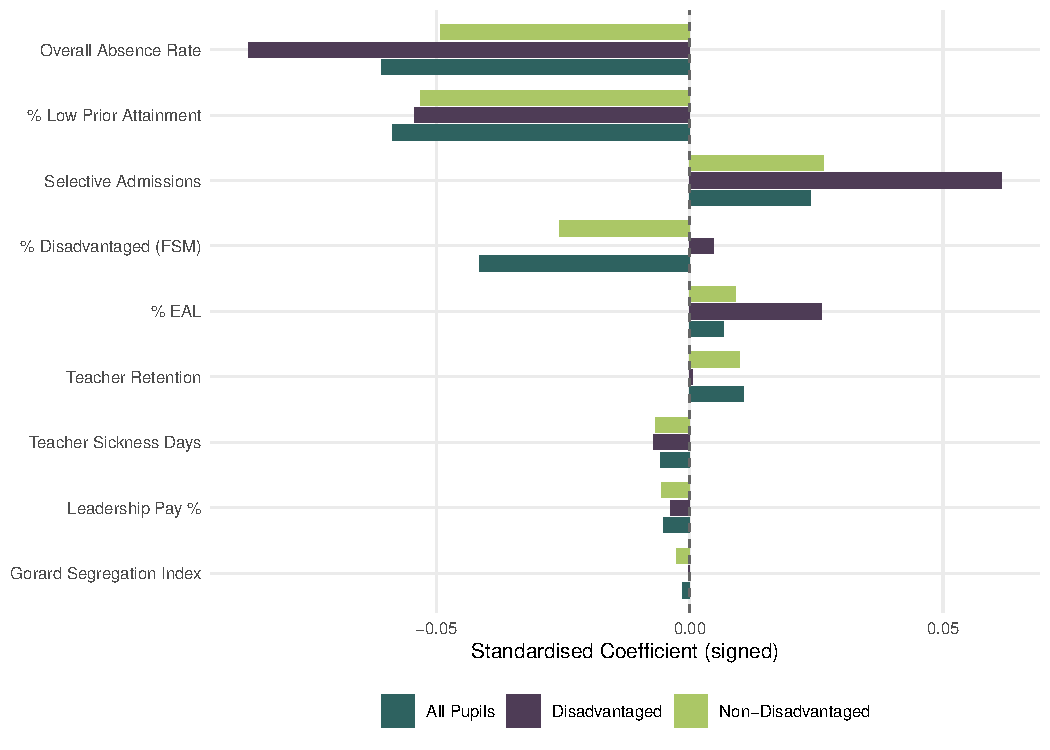
\includegraphics[keepaspectratio]{RPE_Paper_files/figure-pdf/fig-standardised-coefficients-1.pdf}}

}

\caption{\label{fig-standardised-coefficients}Standardised coefficients
showing relative variable importance across pupil groups. Bars show the
change in log(ATT8) associated with a one-SD shift in each predictor.}

\end{figure}%

\begin{figure}

\centering{

\pandocbounded{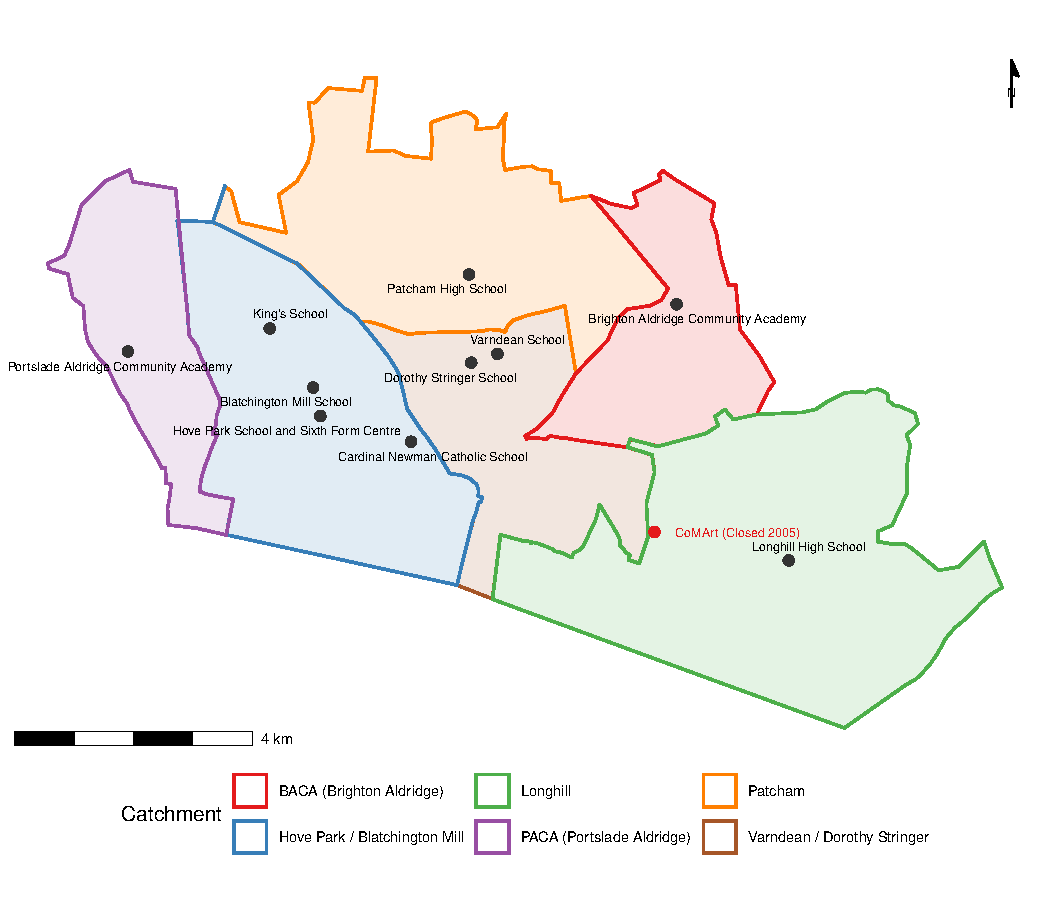
\includegraphics[keepaspectratio]{RPE_Paper_files/figure-pdf/fig-catchments-1.pdf}}

}

\caption{\label{fig-catchments}Brighton and Hove secondary schools with
2025/26 catchment boundaries.}

\end{figure}%

\begin{figure}

\centering{

\pandocbounded{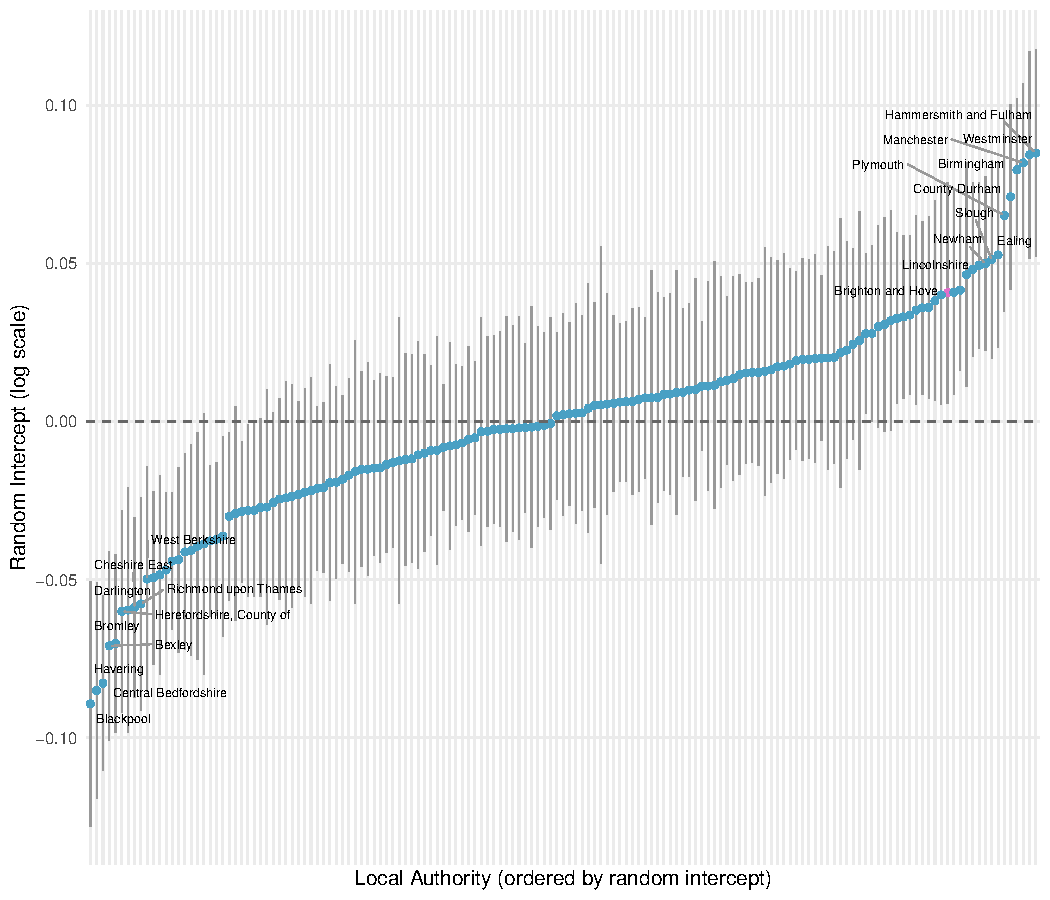
\includegraphics[keepaspectratio]{RPE_Paper_files/figure-pdf/fig-caterpillar-1.pdf}}

}

\caption{\label{fig-caterpillar}LA random intercepts for
disadvantaged-pupil attainment (imputed full panel model). Top and
bottom 10 LAs labelled; Brighton and Hove highlighted.}

\end{figure}%

\begin{longtable}[]{@{}
  >{\raggedright\arraybackslash}p{(\linewidth - 8\tabcolsep) * \real{0.4045}}
  >{\raggedleft\arraybackslash}p{(\linewidth - 8\tabcolsep) * \real{0.1236}}
  >{\raggedleft\arraybackslash}p{(\linewidth - 8\tabcolsep) * \real{0.1798}}
  >{\raggedright\arraybackslash}p{(\linewidth - 8\tabcolsep) * \real{0.1910}}
  >{\raggedleft\arraybackslash}p{(\linewidth - 8\tabcolsep) * \real{0.1011}}@{}}

\caption{\label{tbl-la-absence}Brighton and Hove's local-authority
effect for disadvantaged-pupil attainment, with and without a control
for school absence. The intake-predicted specification controls only for
the part of absence that intake predicts, leaving the city's excess
absence in the residual.}

\tabularnewline

\toprule\noalign{}
\begin{minipage}[b]{\linewidth}\raggedright
Specification
\end{minipage} & \begin{minipage}[b]{\linewidth}\raggedleft
B\&H effect
\end{minipage} & \begin{minipage}[b]{\linewidth}\raggedleft
95\% CI
\end{minipage} & \begin{minipage}[b]{\linewidth}\raggedright
Rank
\end{minipage} & \begin{minipage}[b]{\linewidth}\raggedleft
ATT8 pts
\end{minipage} \\
\midrule\noalign{}
\endhead
\bottomrule\noalign{}
\endlastfoot
No absence control & +0.006 & -0.034 to 0.046 & 69 of 151 (n.s.) &
+0.2 \\
Absence controlled (main model) & +0.041 & 0.006 to 0.076 & 15 of 151 &
+1.6 \\
Intake-predicted absence controlled & +0.005 & -0.035 to 0.044 & 71 of
151 (n.s.) & +0.2 \\

\end{longtable}

\begin{figure}

\centering{

\pandocbounded{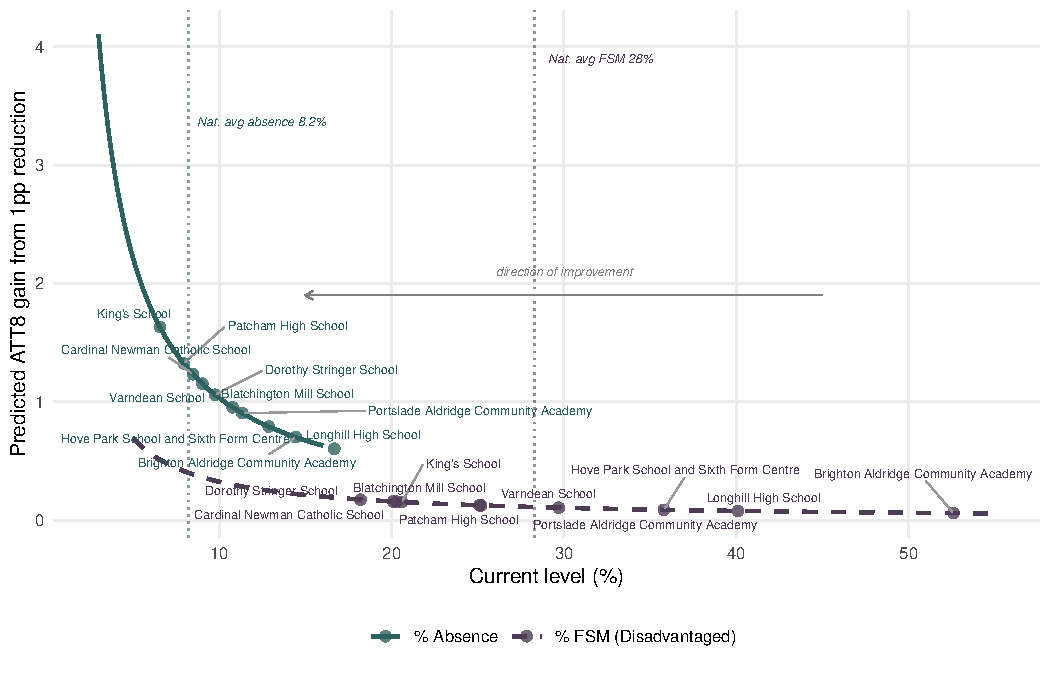
\includegraphics[keepaspectratio]{RPE_Paper_files/figure-pdf/fig-accelerating-returns-1.pdf}}

}

\caption{\label{fig-accelerating-returns}Accelerating returns: each
percentage-point reduction buys a progressively larger ATT8 gain
(reading right to left). Absence delivers substantially larger gains
than FSM at every level. Brighton and Hove schools marked on each
curve.}

\end{figure}%

\begin{figure}

\centering{

\pandocbounded{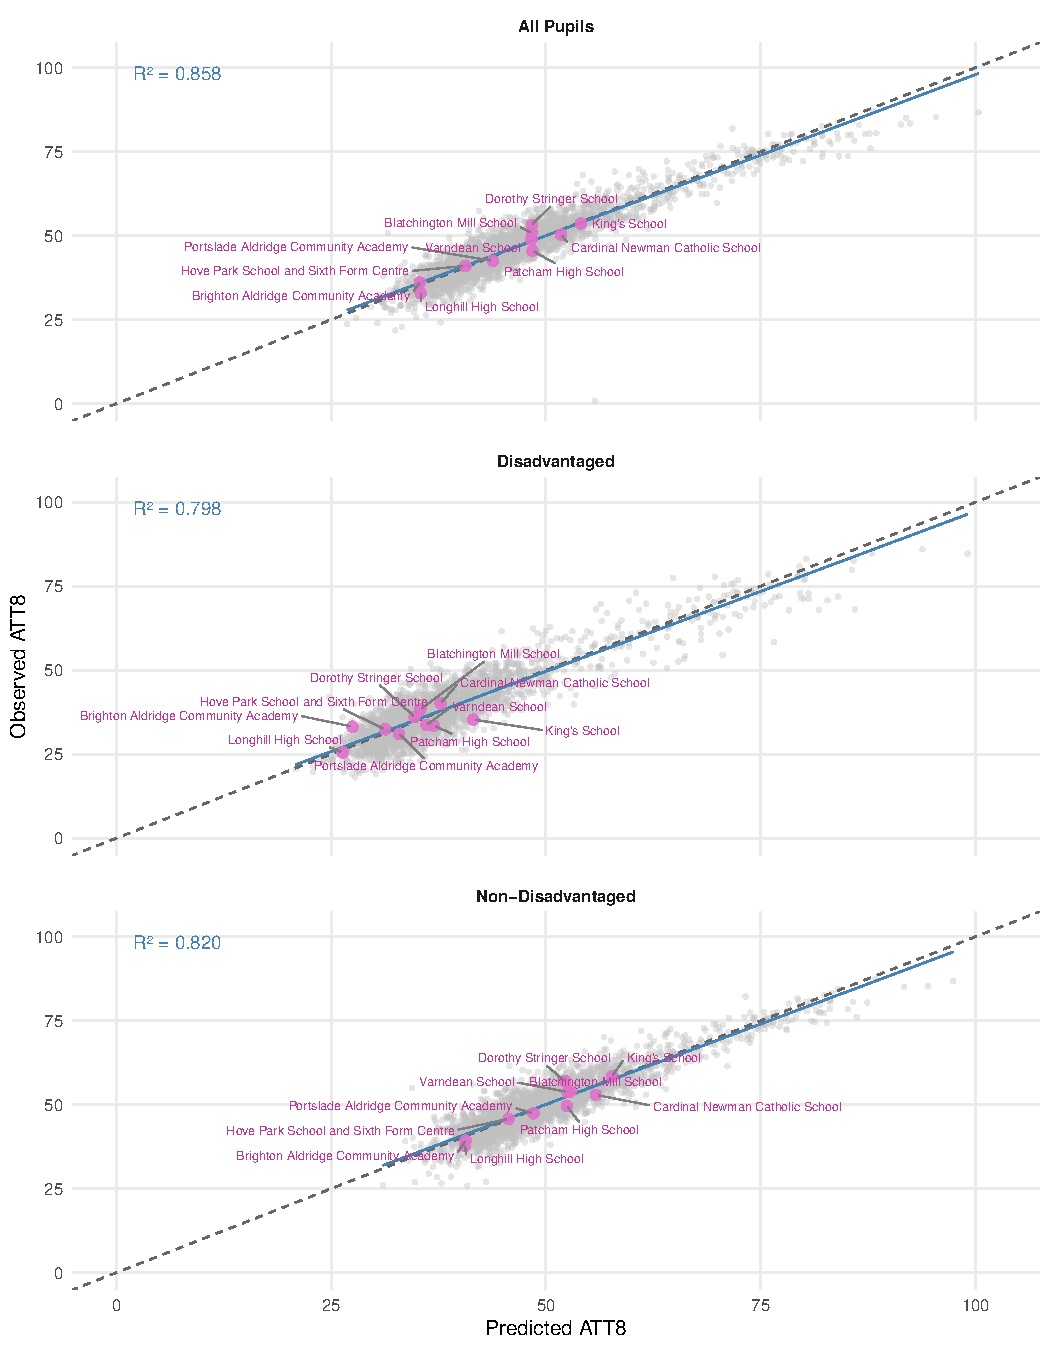
\includegraphics[keepaspectratio]{RPE_Paper_files/figure-pdf/fig-obs-vs-pred-1.pdf}}

}

\caption{\label{fig-obs-vs-pred}Observed versus predicted Attainment 8
for Brighton and Hove schools (highlighted) against all schools
nationally, 2024--25.}

\end{figure}%

\begin{figure}

\centering{

\pandocbounded{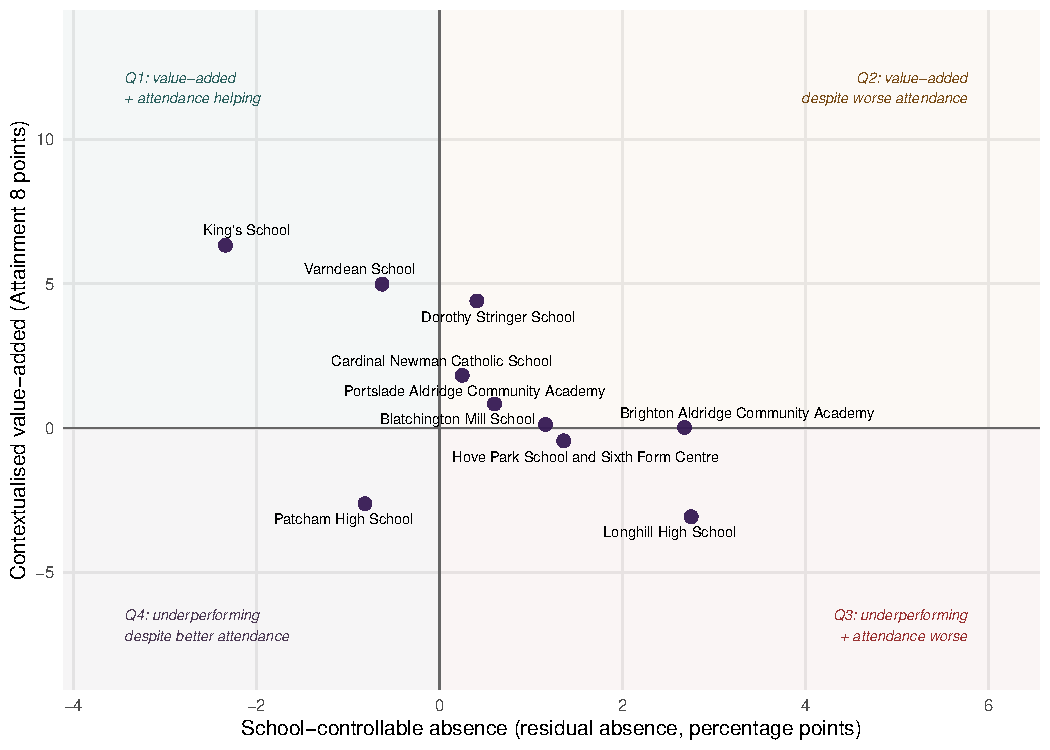
\includegraphics[keepaspectratio]{RPE_Paper_files/figure-pdf/fig-quadrant-1.pdf}}

}

\caption{\label{fig-quadrant}Brighton and Hove secondaries on the
joint-signal plane: contextualised value-added (vertical, in Attainment
8 points) versus the school-controllable absence component (horizontal,
in percentage points). The reference lines at zero on each axis split
the plane into four narrative quadrants discussed in the text. The full
national version with a local-authority filter is available
interactively in the project's HTML report.}

\end{figure}%

\begin{table}

\caption{\label{tbl-league}Value-added rankings for Brighton and Hove
schools (panel model residuals by year, in Attainment 8 points).}

\centering{

\centering\begingroup\fontsize{8}{10}\selectfont

\resizebox{\ifdim\width>\linewidth\linewidth\else\width\fi}{!}{
\begin{tabular}[t]{rlrrrr>{}r}
\toprule
Rank & School & 2021-22 & 2022-23 & 2023-24 & 2024-25 & Mean\\
\midrule
\addlinespace[0.3em]
\hline
\multicolumn{7}{l}{\textit{\textbf{All Pupils}}}\\
\hspace{1em}1 & Dorothy Stringer School & +2.5 & +3.1 & +2.2 & +4.8 & \textbf{+3.1}\\
\hspace{1em}2 & Varndean School & +2.7 & +2.6 & +5.3 & +0.5 & \textbf{+2.8}\\
\hspace{1em}3 & King's School & +3.5 & +0.9 & +5.0 & -0.5 & \textbf{+2.2}\\
\hspace{1em}4 & Brighton Aldridge Community Academy & +2.0 & +1.4 & +1.2 & +0.8 & \textbf{+1.4}\\
\hspace{1em}5 & Portslade Aldridge Community Academy & +3.8 & +0.6 & +2.3 & -1.3 & \textbf{+1.4}\\
\hspace{1em}6 & Hove Park School and Sixth Form Centre & +1.5 & +0.9 & +1.4 & +0.4 & \textbf{+1.0}\\
\hspace{1em}7 & Blatchington Mill School & -1.5 & -1.0 & +2.0 & +2.4 & \textbf{+0.5}\\
\hspace{1em}8 & Cardinal Newman Catholic School & +1.3 & -2.2 & +1.3 & -1.5 & \textbf{-0.3}\\
\hspace{1em}9 & Longhill High School & -0.2 & -2.3 & -1.1 & -2.5 & \textbf{-1.5}\\
\hspace{1em}10 & Patcham High School & -2.7 & -2.8 & -4.4 & -2.9 & \textbf{-3.2}\\
\addlinespace[0.3em]
\hline
\multicolumn{7}{l}{\textit{\textbf{Disadvantaged Pupils}}}\\
\hspace{1em}1 & Brighton Aldridge Community Academy & +3.1 & -1.3 & +4.6 & +5.7 & \textbf{+3.1}\\
\hspace{1em}2 & Varndean School & +2.2 & +3.2 & +3.9 & -2.4 & \textbf{+1.7}\\
\hspace{1em}3 & Cardinal Newman Catholic School & +2.9 & -5.4 & +6.5 & +2.3 & \textbf{+1.6}\\
\hspace{1em}4 & Dorothy Stringer School & +2.2 & +2.6 & -0.2 & +1.4 & \textbf{+1.5}\\
\hspace{1em}5 & Blatchington Mill School & -5.0 & +1.1 & +4.7 & +2.9 & \textbf{+0.9}\\
\hspace{1em}6 & King's School & +4.8 & +1.4 & +3.8 & -6.2 & \textbf{+0.9}\\
\hspace{1em}7 & Hove Park School and Sixth Form Centre & +3.0 & -2.5 & +2.0 & +1.1 & \textbf{+0.9}\\
\hspace{1em}8 & Portslade Aldridge Community Academy & +3.2 & -3.4 & +4.1 & -1.9 & \textbf{+0.5}\\
\hspace{1em}9 & Patcham High School & +4.1 & +1.5 & -11.6 & -3.5 & \textbf{-2.4}\\
\hspace{1em}10 & Longhill High School & -5.1 & -6.4 & +1.4 & -0.9 & \textbf{-2.7}\\
\bottomrule
\end{tabular}}
\endgroup{}

}

\end{table}%




\end{document}
